%%%%%%%%%%%%%%%%%%%%%%%%%%%%%%%%%%%%%%%%%%
%+ Chuong 2. Phuong phap phan ra Dantzig-Wolfe giai bai toan QHTT kich thuoc lon, co cau truc.
%+ Modified: 17-05-2008
%%%%%%%%%%%%%%%%%%%%%%%%%%%%%%%%%%%%%%%%%%
\setcounter{chapter}{1}
\begin{flushright}
\chapter{\textbf{OTOMAT VÀ HỮU HẠN VÀ NGÔN NGỮ CHÍNH QUY}}
\end{flushright}
\begin{flushleft}
\hspace{10mm}Trong chương này, chúng ta sẽ nghiên cứu một mô hình $"$máy trừu tượng$"$ để đoán nhận ngôn ngữ, đó là các otomat hữu hạn. Chúng ta sẽ thấy rằng lớp ngôn ngữ được đoán nhận bởi otomat hữu hạn khá đơn giản, đó chính là lớp ngôn ngữ chính quy do văn phạm chính quy sinh ra. Chương này các nội dung chủ yếu sau:\\ 
$\S1.$ Otomat hữu hạn đơn định\\
\hspace{10mm}2.1. Otomat hữu hạn đơn định\\
\hspace{10mm}2.2. Biểu diễn otomat hữu hạn đơn định\\
\hspace{10mm}2.3. Ngôn ngữ được đoán nhận bởi otomat đơn định\\
$\S2.$ Otomat hữu hạn không đơn định\\
\hspace{10mm}3.1. Otomat hữu hạn không đơn định\\
\hspace{10mm}3.2. Ngôn ngữ đoán nhận bởi otomat không đơn định\\
\hspace{10mm}3.3. Đơn định hoá các otomat\\
\hspace{10mm}3.3. Sự tương đương giữa các otomat đơn định và không đơn định\\
$\S3.$ Ngôn ngữ chính quy và biểu thức chính quy\\
\hspace{10mm}4.1. Ngôn ngữ chính quy và biểu thức chính quy\\
\hspace{10mm}4.2. Sự liên hệ giữa otomat hữu hạn và ngôn ngữ chính quy\\
$\S4$. Điều kiện cần của ngôn ngữ chính quy\\
\hspace{10mm}5.1. Otomat tối tiểu\\
\hspace{10mm}5.2. Điều kiện cần của ngôn ngữ chính quy\\
\section{Otomat hữu hạn đơn định}
\textbf{Mở đầu}\\
\hspace{10mm}Một otomat hữu hạn là một mô hình tính toán thực sự hữu hạn. Mọi các liên quan đến nó đều có kích thước hữu hạn cố định và không thể mở rộng trong suốt quá trình tính toán. Các loại otomat khác đươc nghiên cứu sau này có ít nhất một bộ nhớ vô hạn về tiềm năng. Sự phân biệt giữa các loại otomat khác nhau chủ yếu dựa trên việc thông tin có thể được đưa và bộ nhớ như thế nào.\\
Một otomat hữu hạn làm việc theo thời gian rời rạc như tất cả các mô hình tính toán khác. Như vậy, ta có thể nói về thời điểm "kế tiếp" khi "đặc tả" hoạt động 
của một otomat hữu hạn.\\
Trường hợp đơn giản nhất là thiết bị không có bộ nhớ mà ở mỗi thời điển, thông tin chỉ phụ thuộc vào thông tin vào lúc đó. Các thiết bị như vậy là mô hình của các mạch tổ hợp.\\
Tuy nhiên, nói chung, thông tin ra sản sinh bởi một otomat hữu hạn phụ thuộc vào cả thông tin vào hiện tại lẫn các thông tin vào trước đó. Như vậy otomat có khả năng (với một phạm vi nào đó) ghi nhớ các thông tin vào trong quá khứ của nó. Một cách chi tiết hơn, điều đó có nghĩa như sau.\\
Mỗi otomat có một số hữu hạn trạng thái được lưu ở bộ nhớ trong. Tại mỗi thời điểm i, nó ở một trong các trạng thái đó, chẳng hạn $q_i$. Trạng thái $q_i$ ở thời điểm sau được xác định bởi $q_i$ và thông tin vào $a_i$ cho ở thời điểm i. Thông tin ra ở thời điểm i được xác định bởi trạng thái $q_i$ (hay bởi cả $a_i$ và $q_i$).\\

\subsection{Otomat hữu hạn đơn định}

\textbf{\textit{Định nghĩa 1.1.}} Một otomat hữu hạn đơn định (Deterministic Finite Automata-DFA) là một bộ năm:
\end{flushleft}
$A = <Q, \sum, \delta, q_0, F>$,
\begin{flushleft}
Trong đó: \\
+ Q là một tập hữu hạn khác rỗng, được gọi là tập các trạng thái;\\
+ $\sum$ là một bảng chữ cái, được gọi là bảng chữ vào;\\
+ $\delta$: $D \to Q$, là một ánh xạ từ D vào Q, trong đó $D \subseteq Q \times \sum$, được gọi là hàm chuyển trạng thái (hay hàm chuyển);\\
+ $q_0 \in Q$, được gọi là trạng thái khởi đầu;\\
+ $D \subseteq Q$ được gọi là tập các trạng thái kết thúc.\\
\hspace{10mm}Trong trường hợp $D = Q \times \sum$, ta nói  ta nói A là otomat đầy đủ. Sau này ta sẽ thấy rằng mọi otomat hữu hạn đều đưa về được otomat hữu hạn đầy đủ tương đương.\\
Hoạt động của otomat hữu hạn đơn định $A = <Q, \sum, \delta, q_0, F>$ khi cho xâu vào $w = a_1a_2...a_n$ có thể được mô tả như sau:\\
\hspace{10mm}Khi bắt đầu làm việc, otomat ở trạng thái khởi đầu $q_0$ và đầu đọc đang nhìn vào ô có ký hiệu $a_1$. Tiếp theo otomat chuyển từ trạng thái $q_0$ dưới tác động của ký hiệu vào $a_1$ về trạng thái mới $\delta(q_0, a_1) = q_1 \in Q$ và đầu đọc chuyển sang phải một ô, tức là nhìn vào ô có ký hiệu $a_2$. Sau đó otomat A có thể lại tiếp tục chuyển từ trạng thái $q_1$ nhờ hàm chuyển $\delta$ về trạng thái mới $q_2 = \delta(q_1, a_2) \in Q$. Quá trình đó sẽ tiếp tục cho tới khi gặp một trong các tình huống sau:\\
- Otomat A đọc hết xâu vào $w$ và  và $\delta(q_0, a_1) = q_n \not \in F$, ta nói A không đoán nhận xâu $w$.
- Hoặc khi otomat A đọc đến $a_j$ , $(j \le n)$ và hàm $\delta(q_{j-1}, a_j)$ không xác định, ta cũng nói A không đoán nhận $w$.
\end{flushleft}
\begin{center}
\begin{figure}[ht]
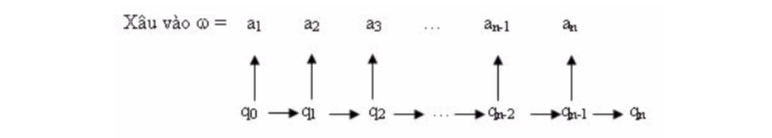
\includegraphics[scale=0.5]{3_1.png}
\caption{ \textit{H. 3.1. Mô tả quá trình đoán nhận xâu $w$ của otomat A} }
\end{figure}
\end{center}

\begin{flushleft}
\subsection{Biểu diễn otomat hữu hạn đơn định}
\hspace{10mm}Hàm chuyển trạng thái là một bộ phận quan trọng của một otomat hữu hạn đơn định. Cho một otomat thực chất là cho hàm chuyển trạng thái của nó, có thể cho dưới dạng bảng chuyển cho dưới dạng đồ thị chuyển.\\
\textbf{Cho otomat bằng bảng chuyển}\\
Cho otomat $A = <Q, \sum, \delta, q_0, F>$ với $Q = \{ q_0, q_1, q_2,...,q_m \}$ là tập trạng thái, và bảng chữ
cái $\sum = \{ a_1, a_2,...,a_n \}$, khi đó hàm chuyển có thể cho bởi bảng sau; trong đó dòng i cột j của
bảng là ô trống nếu $(q_i, a_j) \not \in D$, tức là $\delta(q_i, a_i)$ không xác định. 
\begin{figure}[ht]
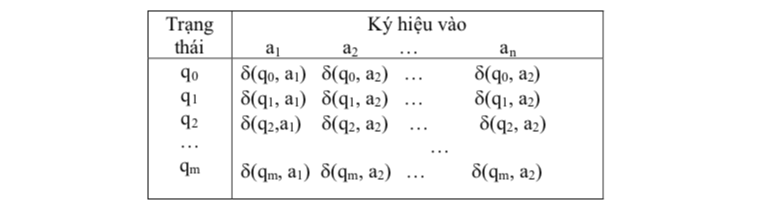
\includegraphics[scale=0.5]{3_2.png}
\caption{ \textit{Bảng chuyển trạng thái của otomat A} }
\end{figure}
\end{flushleft}

\begin{flushleft}
Cho bảng chuyển trạng thái, và chỉ rõ tập trạng thái kết thúc F, ta sẽ xác định được otomat A\\
\textbf{Cho otomat bằng đồ thị chuyển}\\
cho otomat  $A = <Q, \sum, \delta, q_0, F>$. Hàm chuyển $\delta$ có thể cho bằng một đa đồ thị có hướng, có khuyên G sau đây, được gọi là đồ thị chuyển của otomat A. Tập đỉnh của G được gán nhãn bởi các phần tử thuộc Q, còn các cung được gán nhãn bởi các phần tử thuộc $\delta$, tức là nếu $a \in \delta$ và từ trạng thái q chuyển sang trạng thái p theo công thức $\delta = (q,a) = p$ thì sẽ có một cung từ đỉnh q tới đỉnh p được gán nhãn a.\\
Đỉnh vào của đồ thị chuyển là đỉnh ứng với trạng thái ban đầu $q_0$. Các đỉnh sẽ được khoanh bởi các vòng tròn, tại đỉnh $q_0$ có mũi tên đi vào, riêng đỉnh với trạng thái kết thúc được phân biệt bởi vòng tròn đậm, hoặc hình vuông…\\
Nói chung, với việc cho đồ thị chuyển là hoàn toàn xác định được otomat A.\\
\textbf{Thí dụ 1.1 } Cho hai otomat hữu hạn đơn định:\\
1/. $A_1 = <\{ q_0, q_1, q_2 \}, \{ a,b \}, \delta, q_0, \{ q_2 \}>$,\\
với $\delta(q_0, a) = q_0, \delta(q_0, b) = q_1, \delta(q_1, a) = q_0, \delta(q_1, b) = q_2, \delta(q_2, a) = q_2, \delta(q_2, b)=q_2$.
Ta có bảng chuyển trạng thái và đồ thị chuyển trạng thái của otomat A1 như sau:\\
\begin{figure}[ht]
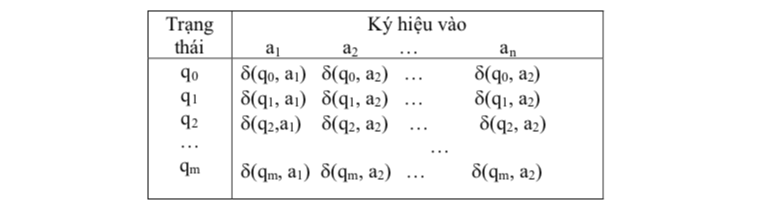
\includegraphics[scale=0.5]{3_3.png}
\caption{ \textit{ Bảng chuyển trạng thái của A1} }
\end{figure}

\begin{figure}[ht]

\includegraphics[scale=0.5]{3_4.png}
\caption{ \textit{Đồ thị chuyển trạng thái $A_1$} }
\end{figure}
Dãy trạng thái của otomat A1 trong quá trình đoán nhận xâu vào $\delta = ababbab$ là:\\
\begin{figure}[ht]
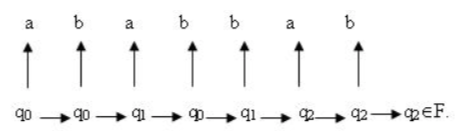
\includegraphics[scale=0.5]{3_5.png}
\caption{ \textit{Quá trình đóan nhận xâu $\delta = ababbab$ của $A_1$} }
\end{figure}
Như vậy, xâu $\delta$ được đoán nhận bởi otomat $A_1$.\\
2/. $A_2 = <\{q_0,q_1,q_2,q_3\}, \{0,1\}, \delta, q_0, \{q_0\}>$, \\
trong đó $\delta(q_0, 0) = q_2, \delta(q_0, 2) = q_1, \delta(q_1, 0) = q_3, \delta(q_1, 1) = q_0, \delta(q_2, 0) = q_0, \delta(q_2, 1) = q_3, \delta(q_3, 0) = q_1, \delta(q_3, 1) = q_2$.
Ta có bảng chuyển trạng thái và đồ thị chuyển trạng thái của otomat $A_2$ được cho trong hình 3.6 và 3.7: 
\begin{figure}[ht]
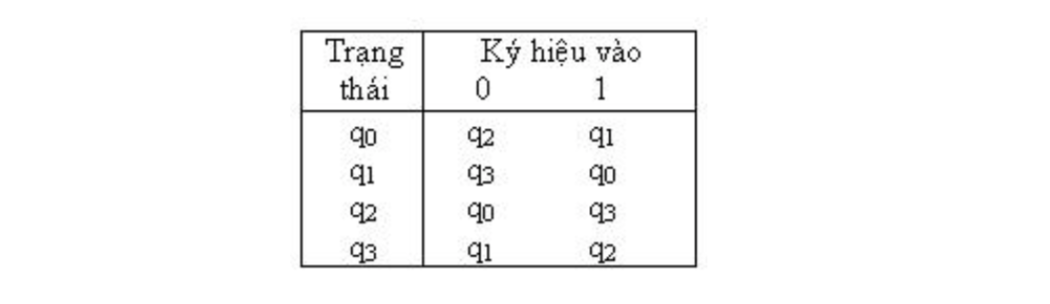
\includegraphics[scale=0.4]{3_6.png}
\caption{ \textit{Bảng chuyển trạng thái của $A_2$} }
\end{figure}

\begin{figure}[ht]
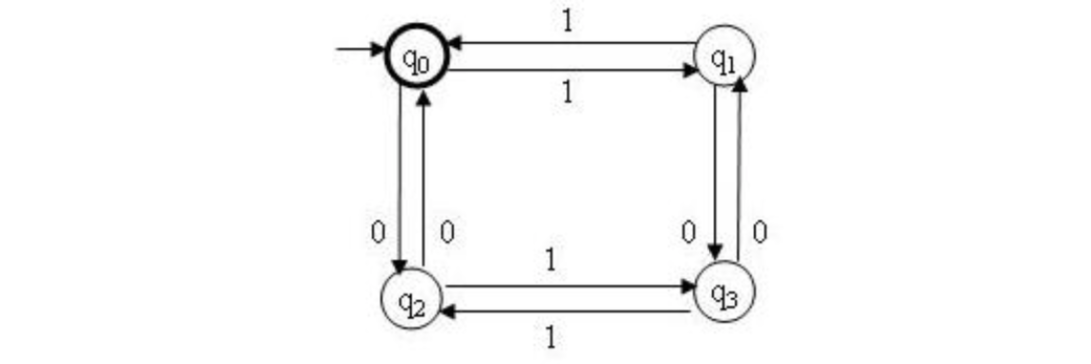
\includegraphics[scale=0.4]{3_7.png}
\caption{ \textit{Đồ thị chuyển trạng thái của $A_1$} }
\end{figure}
\end{flushleft}

\begin{figure}[ht]
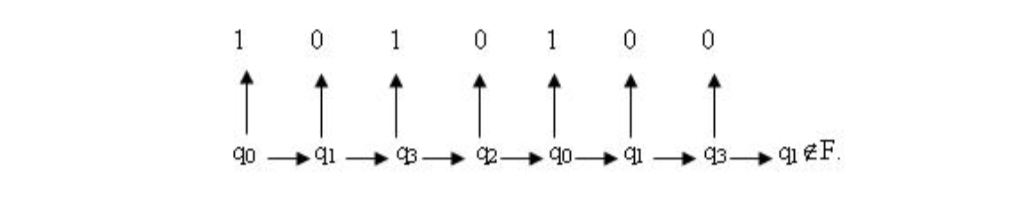
\includegraphics[scale=0.5]{3_8.png}
\caption{ \textit{Qúa trình đoán nhận xâu vào $\beta$ = 1010100} }
\end{figure}

\begin{flushleft}
Dãy trạng thái của otomat A2 trong quá trình đoán nhận xâu vào $\beta$ = 1010100 là:
\end{flushleft}

\begin{flushleft}
Như vậy, otomat A2 không chấp nhận xâu $\beta$.\\
Ta có thể mô tả quá trình đoán nhận xâu vào của otomat hữu hạn đơn định đầy đủ A bằng thuật toán mô phỏng sau:\\
\hspace{10mm} \textbf{Input}:\\
\hspace{10mm} - Một xâu $w$, kết thúc bởi ký hiệu kết thúc file là eof.\\
\hspace{10mm} - Một otomat hữu hạn đơn định đầy đủ A với trạng thái đầu $q_0$ và tập trạng thái kết thúc là F.\\
\hspace{10mm} \textbf{Output}:\\
\hspace{10mm} - Trả lời “Đúng” nếu A đoán nhận xâu $w$.\\
\hspace{10mm} - Trả lời “Sai” nếu A không đoán nhận xâu $w$.\\
\hspace{10mm} \textbf{Thuật toán}:\\
Begin\\
\hspace{10mm} S:= $q_0$;\\
\hspace{10mm} C:= ký hiệu tiếp theo;\\
\hspace{10mm} While C < > eof do\\
\hspace{20mm} begin\\
\hspace{30mm} S:= $\delta$(S, C);\\
\hspace{30mm} C:= ký hiệu tiếp theo;\\
\hspace{20mm} end;\\
\hspace{10mm} if S in F return (True)\\
\hspace{10mm} else return (False);\\
End.\\
\textbf{1.3 Ngôn ngữ được đoán nhận bởi otomat đơn định}\\
Để mô tả hình thức quá trình đoán nhận một từ (xâu vào), người ta đưa vào ánh xạ mở rộng $\delta'$ từ $D \subseteq q \times \sum^*$ vào Q như trong định nghĩa sau: \\
\textbf{Định nghĩa 1.2} Cho otomat hữu hạn đơn định $A = <Q, \sum, \delta, q_0, F>$. Mở rộng $\delta$ của $\delta$ là một ánh xạ từ $D \subseteq Q \times \sum^*$ vào Q được xác định như sau: \\
1/. $\delta(q, \varepsilon) = q, \forall q \in Q$,\\
2/. $\delta(q, wa) = \delta(\delta(q, w), a), \forall a \in \sum, \forall q\in Q, \forall w \in Q, \forall w \in \sum^*$ sao cho $\delta(q, w)$ được xác định.\\
Chú ý rằng, ánh xạ $\delta$ chỉ khác ánh xạ $\delta'$ khi ký hiệu vào là $\varepsilon$, hoặc là một xâu kí hiệu vào $w$, do điều kiện 2/. trên $Q \times \sum$ , ta có thể đồng nhất $\delta'$ với $\delta$. Nếu không cần phân biệt, từ đây về sau ta viết $\delta$ thay cho $\delta'$, và được hiểu là ánh xạ $\delta$ trên miền $Q \times \sum$ , là ánh xạ $\delta'$ trên miền $Q \times \sum^*$.\\
\textbf{Định nghĩa 1.3} Cho otomat hữu hạn đơn định $A = <Q, \sum, \delta, q_0, F>$, và một xâu $w \in \sum^*$. Ta nói:\\
+ $w$ được đoán nhận bởi A nếu $\delta(q_0, w) \in F$;\\
+ Ngôn ngữ được đoán nhận bởi otomat A và ký hiệu là T(A), là tập từ:\\
$T(A) = {w \in sum^* | \delta(q_0, w) \in F}$\\
Lưu ý rằng trong đồ thị chuyển của A, $w \in \sum^*$ được đoán nhận bởi A khi và chỉ khi $w$ là xâu của các nhãn ứng với một đường đi từ đỉnh $q_0$ đến một trong các đỉnh kết thúc. Cụ thể, nếu $w= a_1a_2...a_n$ thì đường đi là $(q_0, q_1,..., q_k)$ với cung $(q_i-1, q_i)$ có nhãn $a_i$ (với $1 \le i \le k$) và $q_k \in F$.\\
Như vậy, T(A) là tập hợp tất cả xâu ghi trên các đường đi từ $q_0$ đến các đỉnh kết thúc.\\
\textbf{Định nghĩa 1.4} Hai otomat hữu hạn $A = <Q, \sum, \delta, q_0, F> và A'= <Q', \sum', \delta', q'_0, F'>$ được gọi là tương đương nếu $T(A) = T(A')$.\\
\textbf{Thí dụ 1.2} Cho otomat hữu hạn: $A_3 = <{q_0, q_1, q_2, q_3, q_4},{0, 1}, \delta, q_0, {q_1, q_2, q_4}>$ với $\delta(q_0,0) = q_0, \delta(q_0,1) = q_1, \delta(q_1,0) = q_3, \delta(q_1,1) = q_2, \delta(q_2,0) = q_2, \delta(q_2,1) = q_2, \delta(q_3,1) = q_3, \delta(q_4,0) = q_2, \delta(q_4,1) = q_3.$.\\
\hspace{10mm}Đồ thị chuyển của A3 là:\\
\begin{figure}[ht]
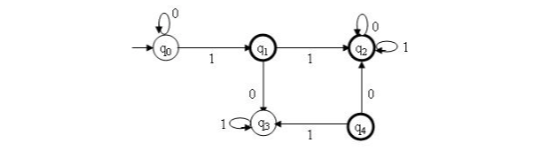
\includegraphics[scale=0.5]{3_9.png}
\caption{ \textit{Đồ thị chuyển của otomat $A_3$}}
\end{figure}

Trước hết, ta nhận thấy rằng không có đường đi từ $q_0$ đến đỉnh kết thúc $q_4$, tức là sẽ không có từ nào được đoán nhận bởi $A_3$ với đỉnh kết thúc $q_4$. Ngoài ra, cũng không có một đường đi nào từ $q_0$ đến đỉnh một đỉnh kết thúc mà đi qua $q_3$. Như vậy, ta có thể bỏ đi đỉnh $q_3$ và $q_4$ mà không ảnh hưởng đến việc đoán nhận các từ của otomat $A_3$. Do đó otomat $A_3$ tương đương với otomat $A_4$ sau: \\
$A_4 = <{q_0, q_1, q_2}, {0, 1}, \delta, q_0, {q_1, q_2}>,$\\
trong đó $\delta(q_0,0) = q_0, \delta(q_0,1) = q_1, \delta\delta(q_1,1) = q_2, \delta(q_2,0) = q_2, \delta(q_2,1) = q_2.$.\\
Đồ thị chuyển của $A_4$ được cho trong hình 3.10:\\
\begin{figure}[ht]

\includegraphics[scale=0.5]{3_10.png}
\caption{ \textit{Đồ thị chuyển của otomat $A_4$}}
\end{figure}
Các đường đi từ q0 đến đỉnh kết thúc q1 ứng với các xâu $0^n1, n \le 0$. Các đường đi từ $q_0$ đến đỉnh kết thúc q2 ứng với các xâu $0^n11w, n \le 0, w \in {0, 1}^*$. Vậy ngôn ngữ được đoán nhận bởi các otomat trên là: \\
$T(A_3) = T(A_4) = {0^n1, 0^n11w / n \le 0, w \in {0, 1}^*}.$ \\
\textbf{Bổ đề 1.1} Cho otomat hữu hạn đơn định $A = <Q, \sum, \delta, q_0, F>.$  Khi đó $\forall w_1, w_2 \in \sum^*, \forall q in Q$ sao cho $\delta(q, w_1w_2)$ xác định, ta có:\\
\end{flushleft}
$\delta(q, w1w2) = \delta(\delta(q, w_1), w_2)$\\
\begin{flushleft}
Chứng minh: Ta chứng minh đẳng thức trên bằng quy nạp theo độ dài của $w_2$.\\
+ Khi $|w_2| = 1$ hay $w_2 = a, a \in \sum$, ta có $\delta(q, w_1a) = \delta(\delta(q, w_1),a)$. Đẳng thức (1) đúng.\\
+ Giả sử đẳng thức (1) đúng với mọi $w_2$ có độ dài $\|w_2\| \le n$. Ta cần chứng minh nó cũng đúng với $w_2$ có độ dài $\|w_2\| = n + 1$.  Đặt $w_2 = w_2'a$, với $w_2' \in \sum^*, |w_2'| = n, a \in \sum. $Ta có $\delta(q, w_1w_2)$


Do đó đẳng thức (1) đúng với $w_2$ có độ dài n + 1.\\
Bổ đề được chứng minh.\\
\textbf{Chú ý: } Với otomat hữu hạn đơn định $A = <Q, \sum, \delta, q_0, F>$ bất kỳ, ta luôn có thể xây dựng một otomat hữu hạn đơn định đầy đủ A’ tương đương với A. \\
Thật vậy, lấy $S \not \in Q$ (do đó $S \not \in F$), đặt $Q'= Q \cup \{S\}$ và $\delta': Q' \times \sum \to Q'$ xác định bởi: $\forall q \in Q, \forall a \in \sum, \delta'(q, a) = \delta(q, a)$ nếu $\delta(q, a)$ được xác định, $\delta'(q, a) = S$ nếu $\delta(q, a)$ không được xác định và $\delta'(S, a) = S$. Khi đó A' là otomat hữu hạn đơn định đầy đủ mà T(A') = T(A). \\
Ta thường chọn S = $\O$, và không cần bổ xung S vào Q.\\

\section{Otomat hữu hạn không đơn định}
\subsection{Otomat hữu hạn không đơn định}
\textbf{Định nghĩa 2.1}\\
Một otomat hữu hạn không đơn định (Nondeterministic Finite AutomataNFA) là một bộ năm:\\
\end{flushleft}
$A = <Q, \sum, \delta, q_0, F>$\\
\begin{flushleft}
trong đó $Q, \sum, q_0, F$ như trong định nghĩa 1.1 và $\delta: Q \times \sum \to 2Q$, ở đây $2Q (hay P(Q)$, là ký hiệu tập hợp các tập con của Q) gọi là ánh xạ chuyển.\\
Rõ ràng ở đây ánh xạ $\delta$ là một hàm đa trị (hàm không đơn định), vì vậy otomat A trong định nghĩa trên đây được gọi là không đơn định.\\
Trong trường hợp $\delta(q, a)$ xác định $\forall q \in Q, \forall a \in \sum$, ta nói ôtômát A là đầy đủ.\\
\hspace{10mm}Nếu $\delta(q, a) = {p_1, p_2,..., p_k}$ thì ta nói rằng otomat A ở trạng thái q gặp ký hiệu a thì có thể chuyển đến một trong các trạng thái $p_1, p_2,..., p_k$. Nếu $\delta(q, a) = {p}$ thì ở trạng thái q gặp ký hiệu a, otomat A chỉ chuyển đến một trạng thái duy nhất p. Nếu $\delta$(q, a) khô ng xác định (ta thường viết $\delta(q, a) = \o $) thì ở trạng thái q gặp ký hiệu a, otomat A không thể chuyển đến trạng thái nào, cũng tương tự như với otomat hữu hạn đơn định.\\
\hspace{10mm}Khi bắt đầu làm việc, otomat ở trạng thái đầu $q_0$ và đầu đọc đang nhìn vào ô có ký hiệu $a_1$. Từ trạng thái $q_0$, dưới tác động của ký hiệu vào $a_1$, $\delta$(q0, a1) = {$p_1,..., p_k$}, otomat xác định các trạng thái có thể tiếp theo là $p_1,..., p_k$ và đầu đọc chuyển sang phải một ô, tức là nhìn vào ô có ký hiệu $a_2$. Tiếp tục với mỗi $p_i (1 \le i \le k)$ và ký hiệu tiếp theo là $a_2$, các trạng thái tiếp theo có thể đến được là $\delta(p_1, a_2)\cup...\cup \delta(p_k, a_2)$. Quá trình đó sẽ tiếp tục cho tới khi gặp một trong các tình huống sau:\\
+ Trong trường hợp tập trạng thái tiếp theo sau khi đọc $a_j$ nào đó là rỗng hoặc sau khi đọc ký hiệu an là Q' mà $Q' \cap F = \o$, ta nói rằng A không đoán nhận $w$.\\
+ Trường hợp tập trạng thái tiếp theo sau khi đọc ký hiệu an là Q' mà $Q' \cap F \ne \o$, ta nói rằng otomat A đoán nhận $w$.\\
Một otomat hữu hạn không đơn định có thể biểu diễn dưới dạng bảng chuyển hoặc đồ thị chuyển như trong trường hợp otomat hữu hạn đơn định. Nếu $\delta(q, a) = \{p_1, p_2, ..., p_k\}$ thì trong đồ thị chuyển có k cung từ q sang $p_1, ..., p_k$ được ghi cùng một nhãn a. \\
\textbf{Thí dụ 2.1} Cho otomat hữu hạn không đơn định:\\
$A = <{q_0, q_1, q_2, q_3, q_4}, {0, 1}, \delta, q_0, {q_2, q_4}>,$\\
Với $\delta(q_0,0) = \{q_0,q_3\},\delta(q_0, 1) = \{q_0,q_1\}, \delta(q_1, 0) = \O, \delta(q_1, 1) = \{q_2\}, \delta(q_2, 0) = \{q_2\},$\\
$\delta(q_2, 1) = \{q_2\}, \delta(q_3, 0) = \{q_4\}, \delta(q_3,1) = \O, \delta(q_4, 0) = \{q_4\}, \delta(q_4, 1) = \{q_4\}.$\\
Bảng chuyển trạng thái và đồ thị chuyển trạng thái của otomat A cho trong hình 3.11 và 3.12:\\
\begin{figure}[ht]
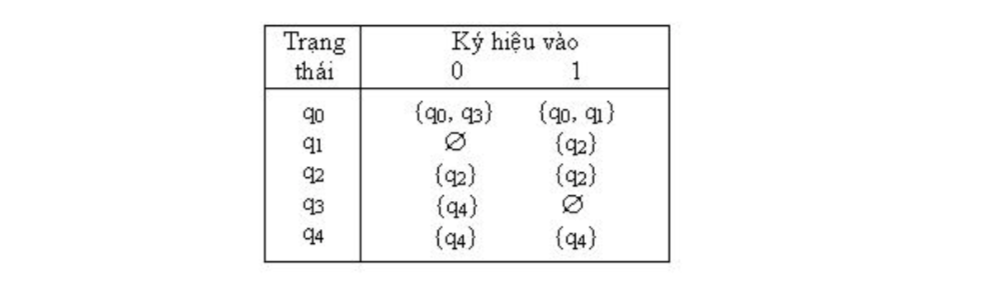
\includegraphics[scale=0.5]{3_11.png}
\caption{ \textit{Bảng chuyển của otomat không đơn định A}}
\end{figure}
\begin{figure}[ht]
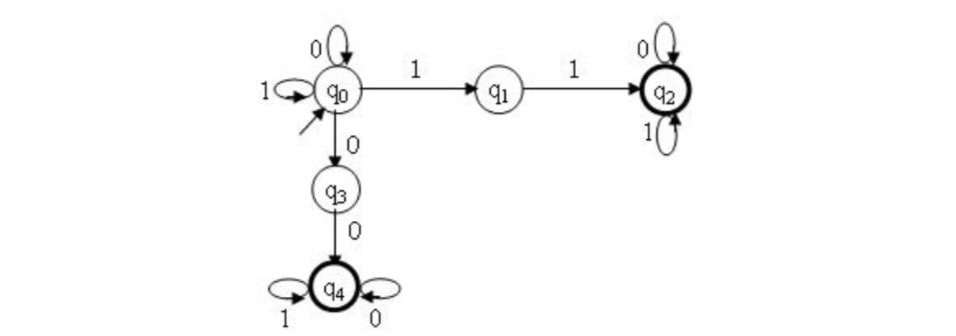
\includegraphics[scale=0.5]{3_12.png}
\caption{ \textit{Đồ thị chuyển của otomat không đơn định A}}
\end{figure}

\textbf{2.2 Ngôn ngữ được đoán nhận bởi otomat hữu hạn không đơn định}\\
\textbf{Định nghĩa 2.2} Cho otomat hữu hạn không đơn định $A = <Q, \sum, \delta, q_0, F>$. Mở rộng của $\delta$ là ánh xạ $\delta'$ từ tập $Q \times \sum^*$ vào 2Q được xác định như sau:\\
1) $\delta'(q, \varepsilon) = \{q\}, \forall q \in \in Q,$\\
2) $\delta'(q, wa) = \sometext_{p \in \delta(q,a)}^{\bigcup}$ $\delta ' ( p, w ) , \forall q\in Q, \forall a \in \sum, \forall w \in \sum^*$ sao cho $\delta'(q, w)$ được xác định.\\
Ta có $\delta'(q, a) = \delta'(q , \varepsilon a) = \sometext_{p \in \delta(q,a)}^{\bigcup} \delta ' ( p, w ) = \sometext_{p \in \delta(q,a)}^{\bigcup} p = \delta(q,a), \forall q \in Q, \forall a \in \sum$, tức là trên $Q \times \sum$ ta có thể đồng nhất $\delta'$ với $\delta$. Vì vậy, cũng như trường hợp otomat hữu hạn đơn định, ta có thể sử dụng ký kiệu $\alpha$ thay cho $\delta'$ và được hiểu là ánh xạ $\delta$ trên miền $Q \times \sum$, là ánh xạ $\delta'$ trên $Q \times \sum^*$.\\
\textbf{Định nghĩa 2.3} Cho otomat hữu hạn không đơn định $A = <Q, \sum, \delta, q_0, F>, w \in \sum^*$ và L là một ngôn ngữ trên $\sum$. Ta nói:\\
- $w$ được đoán nhận bởi A nếu $\delta(q_0, w) \cap F \ne \O$;\\
- L được đoán nhận bởi A nếu $L = \{w \in \sum^* | \delta(q_0, w) \cap F \ne \O\}$ và ký hiệu L là T(A). \\
\textbf{Thí dụ 2.2} Cho otomat hữu hạn không đơn định:\\
$A = <\{q_0, q_1, q_2\}, \{a, b\}, \delta, q_0, \{q_2\}>,$\\
trong đó $\delta(q_0, a) = \{q_0\}, \delta(q_0, b) = \{q_0, q_1\}, \delta(q_1, a) = \{q_1\}, \delta(q_1, b) = \{q_1, q_2\},$\\
\hspace{10mm}$\delta(q2, a) = \{q2\}, \delta(q2, b) = \{q_2\}.$\\
Bảng chuyển và đồ thị chuyển của otomat A được cho trong hình 3.13 và 3.14:\\
\begin{figure}[ht]
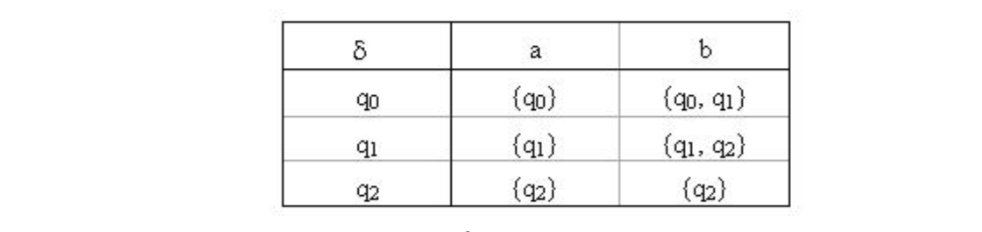
\includegraphics[scale=0.5]{3_13.png}
\caption{ \textit{Bảng chuyển của otomat A trong thí dụ 2.2}}
\end{figure}

\begin{figure}[ht]

\includegraphics[scale=0.5]{3_14.png}
\caption{ \textit{Đồ thị chuyển của otomat A trong thí dụ 2.2}}
\end{figure}
Có thể kiểm tra được rằng từ $w = a^nb^n \in T(A)$, tuy nhiên otomat A không đoán nhận ngôn ngữ $L = \{ a^nb^n | \forall n \ge 1\}.$\\
Ngôn ngữ được đoán nhận bởi otomat A là:\\
$T(A) = \{w_1bw_2bw_3 | w_1, w_2, w_3 \in \{a, b\}^*\}.$\\
\textbf{2.3 Đơn định hóa các otomat}\\
Trước hết ta cần nhắc lại rằng hai ôtômát hữu hạn A và A'(đơn định hay không đơn định) được gọi là tương đương nếu chúng cùng đoán nhận một ngôn ngữ, tức là T(A) = T(A').\\
Giả sử $A = <Q, \sum, \delta, q_0, F>$ là một otomat không đơn định, khi đó ta có thể xây dựng otomat đơn định và đầy đủ M tương đương với otomat A (theo nghĩa cùng đoán nhận một ngôn ngữ). Việc xây dựng M được thực hiện theo thuật toán sau đây, được gọi là thuật toán đơn định hóa otomat.\\
\textbf{Thuật toán đơn định hóa:}\\
\textbf{Input}: Otomat hữu hạn không đơn định $A = <Q, \sum, \delta, q_0, F>$ \\
\textbf{Output:} Otomat hữu hạn đơn định $M = <Q', \sum, \delta', s_0, F'>$\\
\textbf{Phương pháp:} \\
\textit{Bước 1:} Xây dựng hàm hai biến $T: 2^Q \times \sum \to 2^Q$ thỏa mãn các điều kiện:\\
\hspace{10mm} 1/. $\forall q \in Q, \forall a \in \sum $ thì $ T(q, a) = \{q' \in Q | q' = \delta(q, a) \}$\\
\hspace{10mm}2/. $\forall B \subseteq Q mà \delta(q, a) = B, \forall a \in \sum thì T(B, a) = \sometext_{p \in B}^{\bigcup} T(p,a)$\\
\textit{Bước 2:} Xác định tập trạng thái mới $Q' = \{s_0, s_1,..., s_k | k \le 2^{| Q |} -1\}:$\\
\hspace{10mm} 1/. Đặt $s_0 = \{q_0\}, s_1 = \{q_1\},... s_i = \{q_i\} \forall \{q_0\}, \{q_1\},..., \{q_i\} \in Q,$\\
\hspace{10mm}2/. Đặt $s_i+1 = B_1, s_i+2 = B_2,... \forall B_1, B_2 ... \subseteq Q mà \delta(q_j, a) = B_j.$\\
\hspace{10mm}3/. Nếu otomat A là không đầy đủ, đặt $s_k = \O$ và thêm vào hàm chuyển $\delta'$ các giá trị $\delta'(s_k, a)$ = $s_k \forall a \in \sum$ để otomat M là otomat đầy đủ.\\
\hspace{10mm} 4/. Trạng thái khởi đầu của otomat M là $s_0$.\\
\hspace{10mm} 5/. Tập trạng thái kết thúc của otomat M là $F' = \{s \in Q' | s \cap F \ne \O \}$.\\
\textit{Bước 3:} Xác định hàm chuyển $\delta': Q' \times \sum \to Q'$ của otomat M:\\
\end{flushleft}
$\forall s \in Q', \forall a \in \sum $ thì $ \delta'(s, a) = T(s, a)$\\
\begin{flushleft}
Việc chứng minh T(A) = T(M) là khá dễ dàng, dành cho sinh viên như là bài tập.\\
\textbf{Thí dụ 2.3}\\
Cho otomat $A = <{p_0, p_1, p_2}, \{a, b, c\}, \delta , p_0, \{p_1, p_2\}> $với hàm chuyển $\delta$ cho bởi bảng sau:\\
\begin{figure}[ht]
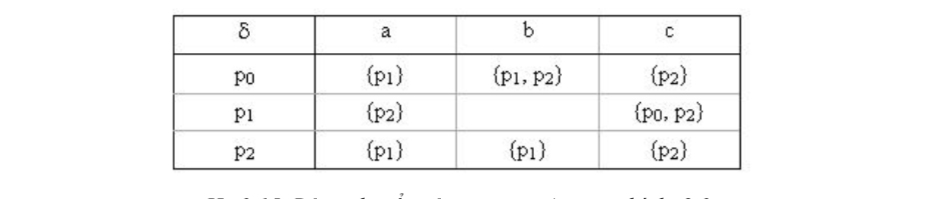
\includegraphics[scale=0.5]{3_15.png}
\caption{ \textit{Bảng chuyển của otomat A trong thí dụ 2.3}}
\end{figure}
Hãy xây dựng otomat $M = <Q', \{a, b, c\}, \delta', s_0, F'>$ đơn định và đầy đủ, tương đương với otomat A.\\
\hspace{10mm}1/. Xây dựng hàm $T: 2Q \times \sum \to 2Q$\\
+ $T(p_0, a) = \{p_1\}, T(p_0, b) = \{p_1, p_2\}, T(p_0, c) = \{p_2\},$\\
+ $T(p_1, a) = \{p_2\}, T(p_1, b) = \O , T(p_1, c) = \{p_0, p_2\},$\\
+ $T(p_2, a) = \{p_1\}, T(p_2, b) = \{p_1\}, T(p_2, c) = \{p_2\},$\\
+ $T(\{p_1, p_2\}, a) = T(p_1,a) \cup T(p_2,a) = \{p_2\} \cup\{p1\} = \{p_1, p_2\}, T(\{p_1, p_2\}, b) = \O \cup \{p_1\} = =\{p_1\}, T(\{p_1, p_2\}, c) = \{p_0, p_2\} \cup \{p_2\} = \{p_0, p_2\},$\\
+ $T(\{p_0, p_2\}, a) = \{p_1\}, T(\{p_0, p_2\}, b) = \{p_1, p_2\}, T(\{p_0, p_2\}, c) = \{p_2\}$\\
\hspace{10mm} 2/. Đặt $s_0 = \{p_0\}, s_1 = \{p_1\}, s2 = \{p_2\}, s_3 = \{p_1, p_2\}, s_4 = \{p_0, p_2\}, s_5 = \O$ ta có:\\
+ Tập trạng thái mới $Q’ = \{s_0, s_1, s_2, s_3, s_4, s_5\}.$\\
+ Trạng thái khởi đầu của M là $s_0$,\\
+ Tập trạng thái kết mới: $F' = \{s_1, s_2, s_3, s_4\}.$\\
\hspace{10mm}3/. Hàm chuyển mới $\delta': Q' \times \sum \to Q'$ được xác định như sau:\\
\begin{figure}[ht]
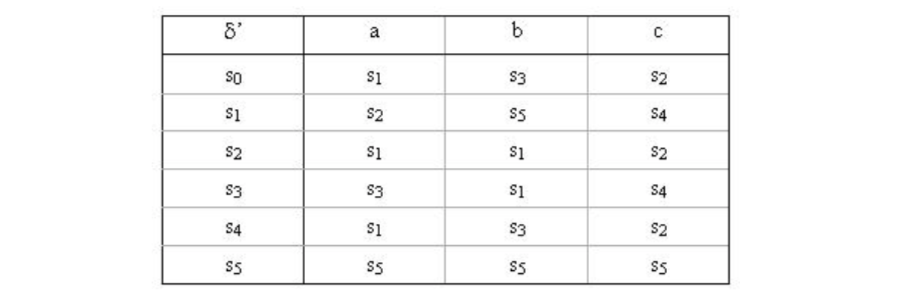
\includegraphics[scale=0.5]{3_16.png}
\caption{ \textit{Bảng chuyển của otomat đơn định M trong thí dụ 2.3}}
\end{figure}
Rõ ràng otomat $M = <{s_0, s_1, s_2, s_3, s_4, s_5}, \{a, b, c\}, \delta', s_0, \{s_1, s_2, s_3, s_4\}>$ với hàm chuyển $\delta'$ cho bởi bảng trên là otomat hữu hạn đơn định và đầy đủ. Có thể thây rằng otomat M là tương đương với otomat A.\\
\textbf{Thí dụ 2.4} Cho otomat không đơn định: $A = <\{q_0, q_1\}, \{a, b\}, delta, q_0, \{q_1\}>, $ trong đó $ delta(q_0, a) = \{q_0\}, \delta(q_0, b) = \{q_0, q_1\}, \delta(q_1, a) = \{q_0, q_1\}, \delta(q_1, b) = \O.$ Đồ thị chuyển của A là:
\begin{figure}[ht]

\includegraphics[scale=0.5]{3_17.png}
\caption{ \textit{Đồ thị chuyển của otomat đơn định M trong thí dụ 2.4}}
\end{figure}
Ta xây dựng otomat $M = <Q', \{a, b\}, \delta', t_0, F'>$ tương đương với A theo thuật toán đơn định hóa, ta có:\\
+ $Q' = \{t_0, t_1, t_2, t_3\}, với t_0 = \{q_0\}, t_1 = \{q_1\}, t_2 = \{q_0, q_1\}, t_3 = \O.$\\
+ $\delta'(t_0, a) = t_0, \delta'(t_0, b) = t_2, \delta'(t_1, a) = t_2, \delta'(t_1, b) = t_3, \delta'(t_2, a) = \{q_0\}\cup \{q_0, q_1\} = t_2, \delta'(t_2, b) = \{q_0, q_1\} \cup \O = t_2, \delta'(t_3, a) = t_3, \delta'(t_3, b) = t_3.$\\
Ta có bảng chuyển của M:
\begin{figure}[ht]
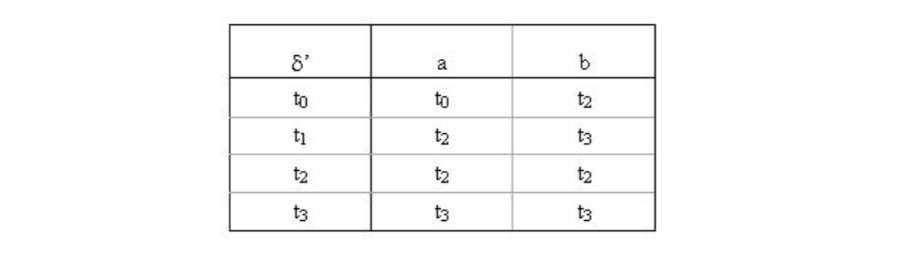
\includegraphics[scale=0.5]{3_18.png}
\caption{ \textit{Bảng chuyển của otomat đơn định M trong thí dụ 2.4}}
\end{figure}
+ Do $t1 \cap F = \{q_1\} \ne \O , t_2 \cap F = \{q1\} \ne \O nên F' = \{t_1, t_2\}.$\\
Rõ ràng otomat M là đơn định và có đồ thị chuyển như sau:\\
\begin{figure}[ht]
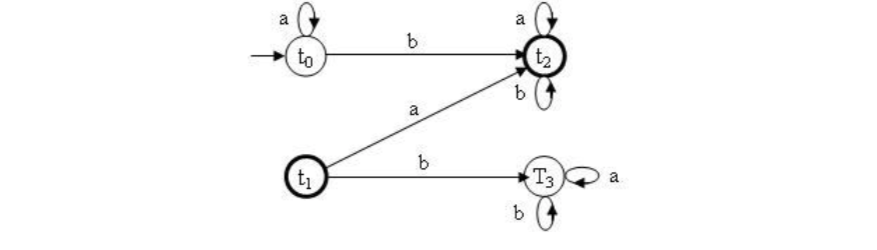
\includegraphics[scale=0.5]{3_19.png}
\caption{ \textit{Đồ thị chuyển của otomat đơn định M trong thí dụ 2.4}}
\end{figure}
Nhìn vào bảng chuyển và đồ thị chuyển của M, ta thấy ngay rằng không có đường đi nào từ $t_0$ đến được đỉnh kết thúc $t_1$, vì vậy otomat M sẽ tương đương với otomat M' có đồ thị chuyển như sau:
\begin{figure}[ht]

\includegraphics[scale=0.5]{3_20.png}
\caption{ \textit{Đồ thị chuyển của otomat M' trong thí dụ 2.4}}
\end{figure}
và ta có $T(A) = T(M) = T(M') = \{a^nbw | n \le 0, w \in \{a, b\}^*\}.$\\
\textbf{2.4 Sự tương đương giữa otomat đơn định và otomat không đơn định}\\
Các định lý dưới đây sẽ cho ta thấy sự tương đương giữa otomat hữu hạn đơn định và không đơn định.\\
\textbf{Định lý 2.1} Nếu ngôn ngữ L được đoán nhận bởi một otomat hữu hạn không đơn định thì tồn tại một otomat hữu hạn đơn định đoán nhận L.\\
Việc chứng minh định lý này được suy từ thuật toán đơn định hóa các otomat.\\
\textbf{Định lý 2.2} 
Lớp ngôn ngữ được sinh bởi otomat hữu hạn đơn định là trùng với lớp ngôn ngữ được sinh bởi otomat hữu hạn không đơn định.\\
\textit{Chứng minh:} Ta gọi LN là lớp ngôn ngữ sinh bởi các otomat hữu hạn không đơn định, LD là lớp ngôn ngữ sinh bởi các otomat hữu hạn đơn định, ta cần chứng minh LN = LD. Ta sẽ chứng minh hai bao hàm thức:\\
\hspace{10mm}$\bullet$ LN $\subseteq$ LD. Giả sử L là một ngôn ngữ tùy ý thuộc lớp LN, tức là tồn tại một otomat không đơn định A đoán nhận L, tức là ta có T(A) = L. Theo định lý 2.1, tồn tại một otomat đơn định M sao cho L = T(M), vậy L thuộc lớp LD, hay LN $\subseteq$ LD.\\
\hspace{10mm}$\bullet$ LD $\subseteq$ LN. Giả sử L là một ngôn ngữ tùy ý thuộc lớp LD, tức là tồn tại một otomat đơn định M đoán nhận L, ta có T(M) = L. Tuy nhiên, ta luôn luôn có thể xem hàm chuyển đơn định $\delta(q, a) = p \in Q$ trong otomat đơn định như là một trường hợp đơn giản của hàm chuyển không đơn định $\delta(q, a) = \{p\} \in 2^Q$ trong otomat không đơn định. Như vậy, một otomat đơn định có thể được xem là một trường hợp đặc biệt của otomat không đơn định. Và vì thế, ngôn ngữ L nói trên có thể xem là được đoán nhận bởi otomat không đơn định. Do đó LD $\subseteq$ LN. \\
\hspace{10mm}Từ đó ta có LD = LN.\\
Định lý được chứng minh.\\
\section{Ngôn ngữ chính quy và biểu thức chính quy}
\hspace{10mm}Trong chương trước, ta đã định nghĩa các ngôn ngữ chính quy thông qua các văn phạm chính quy. Trong phần này, ta sẽ định nghĩa các ngôn ngữ chính quy trực tiếp từ các khái niệm về ngôn ngữ, ta cũng sẽ chỉ ra rằng các định nghĩa này là tương đương. Đồng thời với các ngôn ngữ chính quy, chúng ta đưa ra các khái niệm về biểu thức chính quy, là công cụ để biểu diễn các ngôn ngữ chính quy.\\
\subsection{Ngôn ngữ chính quy và biểu thức chính quy}
\textbf{Định nghĩa 3.1} Cho bảng chữ cái $\sum = \{a_1, a_2,..., a_n\}$, khi đó ngôn ngữ chính quy (regular languages) được định nghĩa đệ quy như sau:\\
\hspace{10mm} 1/. Các ngôn ngữ $\subseteq$ và $\{a_i\} ( i = 1, 2,..., n) $được gọi là các ngôn ngữ chính quy trên bảng chữ cái $\sum$.\\
\hspace{10mm} 2/. Nếu R và S là hai ngôn ngữ chính quy trên bảng chữ cái $\sum$ thì $R \cap S; R.S; R+$ (hay S+) là các ngôn ngữ chính quy trên bảng chữ cái $\sum$.\\
\hspace{10mm}3/. Không có các ngôn ngữ chính quy nào khác trên bảng chữ cái $\sum$ ngoài các ngôn ngữ chính quy được định nghĩa như trên.\\
Có thể thấy rằng định ngghĩa 3.1 trên đây là tương đương với định nghĩa ngôn ngữ chính quy thông qua các văn phạm chính quy. Thật vậy, có thể chỉ ra các văn phạm chính quy sinh ra các ngôn ngữ $\O$ và ngôn ngữ $\{a\}$ (xem thí dụ 4.7, $\S$4, Ch. 1). Ngoài ra, trong chương 1 cũng đã chỉ ra rằng lớp các ngôn ngữ chính quy là đóng đối với các phép toán hợp, nhân ghép và lặp trên các ngôn ngữ. Như vậy lớp ngôn ngữ chính quy được định nghĩa theo định nghĩa trên đây là trùng với lớp ngôn ngữ chính quy đã được định nghĩa theo văn phạm.\\
Như vậy, từ định nghĩa 3.1, ta có định lý sau:\\
\textbf{Định lý 3.1} Mọi ngôn ngữ chính quy trên bảng chữ cái $\sum$ đều nhận được từ các ngôn ngữ hữu hạn bằng cách áp dụng một số hữu hạn lần các phép toán hợp, nhân ghép và phép lặp.\\
\textbf{Chú ý:} \\
1/. Các văn phạm chính quy không chứa các quy tắc sinh từ rỗng (còn gọi là các quy tắc rỗng, là các quy tắc có dạng $A \to \varepsilon$, với A là ký hiệu phụ), vì vậy các ngôn ngữ chính quy cũng không chứa từ rỗng $\varepsilon$.\\
2/. Ngôn ngữ chính quy suy rộng là các ngôn ngữ chính quy có chứa từ rỗng $\varepsilon$, văn phạm chính quy có chứa quy tắc rỗng được gọi là văn phạm chính quy suy rộng\\
Để diễn đạt các ngôn ngữ chính quy, ta đưa vào khái niệm biểu thức chính quy, được định nghĩa như sau:\\
1/. $\O$ và a (với $a \in \sum$) là các biểu thức chính quy trên bảng chữ cái $\sum$ biểu diễn ngôn ngữ $\O$ và ngôn ngữ $\{a\}$\\
2/. Nếu r và s là hai biểu thức chính quy biểu diễn các ngôn ngữ chính quy R và S trên bảng chữ cái $\sum$ thì:\\
\hspace{10mm}$\bullet$ r + s là biểu thức chính quy trên bảng chữ cái $\sum$ biểu diễn ngôn ngữ $R \cup S$\\
\hspace{10mm}$\bullet$ r.s là biểu thức chính quy trên bảng chữ cái $\sum$ biểu diễn ngôn ngữ R.S\\
\hspace{10mm}$\bullet$r+ (hay s+) là biểu thức chính quy trên bảng chữ cái $\sum$ biểu diễn ngôn ngữ R+ (hay S+)\\
3/. Không có các biểu thức chính quy nào khác trên bảng chữ cái $\sum$ ngoài các biểu thức chính quy được định nghĩa như trên.\\
Từ định nghĩa ngôn ngữ chính quy và biểu thức chính quy, ta có các kết quả sau về các ngôn ngữ chính quy:\\
\textbf{Định lý 3.2 }Một ngôn ngữ trên bảng chữ cái $\sum$ là chính quy khi và chỉ khi nó được biểu diễn được bằng một biểu thức chính quy.\\
\textbf{Chú ý:} \\
1/. Biểu thức chính quy suy rộng chấp nhận $\varepsilon$ là biểu thức chính quy biểu diễn ngôn ngữ $\{\varepsilon\}$, và chấp nhận phép toán lặp (*), tức là nếu r là biểu thức chính quy biểu diễn ngôn ngữ chính quy R thì $r^*$ là biểu thức chính quy suy rộng biểu diễn ngôn ngữ chính quy suy rộng $R^*$. Trong hầu hết các trường hợp, khi không cần phân biệt, ta dùng khái niệm "biểu thức chính quy" chung cho cả "biểu thức chính quy" và "biểu thức chính quy suy rộng".\\
2/. Trong các biểu thức chính quy ta có thể bỏ qua các dấu ngoặc và quy ước thứ tự các phép toán là phép lặp, phép nhân ghép và cuối cùng là các phép hợp.\\
Nếu r, s, t là các biểu thức chính quy thì ta có các kết quả sau:\\
\hspace{10mm}$\bullet$r+s = s+r,\\
\hspace{10mm}$\bullet$(r+s)+t = r+(s+t),\\
\hspace{10mm}$\bullet$r+r = r,\\
\hspace{10mm}$\bullet$(rs)t = r(st),\\
\hspace{10mm}$\bullet$r(s+t) = rs+rt, (s+t)r = sr+tr,\\
\hspace{10mm}$\bullet$$\O^* = \varepsilon,$\\
\hspace{10mm}$\bullet$$(r^*)^* = r^*, (r^+)^+ = r^+$\\
Có thể chứng minh các kết quả trên bằng cách chỉ ra rằng hai biểu thức chính quy ở hai vế của mỗi đẳng thức đều biểu diễn cùng một ngôn ngữ chính quy. Xin dành việc chứng minh này cho sinh viên như là bài tập.\\
\textbf{Thí dụ 3.1} Xác định ngôn ngữ chính quy được biểu diễn bởi biểu thức r = $(01^*+02)1.$\\
Ta có:\\
\end{flushleft}
$r = (01^*+02)1 = 01^*1+021,$
\begin{flushleft}
vậy ngôn ngữ chính quy biểu diễn bởi r là: \\
$L (r) = L(01^*1+021) = L(01^*1) \cup L(021) = {01^n , 021 | n \le 1}$\\
\textbf{3.2 Sự liên hệ giữa otomat hữu hạn và ngôn ngữ chính quy}\\
Trong chương trước ta đã thấy rằng với mọi ngôn ngữ chính quy đều tồn tại một văn phạm chính quy sinh ra nó, và ngược lại ngôn ngữ sinh bởi văn phạm chính quy là ngôn ngữ chính quy.\\
Trong phần này, ta sẽ thấy có một sự liên hệ tương tự như vậy giữa otomat hữu hạn và ngôn ngữ chính quy\\
\textbf{Định lý 3.3} Nếu L là một ngôn ngữ chính quy thì tồn tại một otomat hữu hạn không đơn định A đoán nhận L, tức là L = T(A).\\
\textit{Chứng minh:} Giả sử L là ngôn ngữ bởi văn pham chính quy $G = <\sum, \triangle, S, P>, tức là L = L(G).$ Xét otomat hữu hạn không đơn định $A = < Q, \sum, \delta, q_0, F>$, trong đó:\\
+ $Q = \triangle \cup \{E\}$, với E là ký hiệu mới và $E \not \in \sum \cup \triangle$,\\
+$ q_0 = S$;\\
+ $F = \{E\}$ nếu quy tắc $S \to \varepsilon \not \in P $ và $ F = \{E, S\}$ nếu $S \to \varepsilon \in P$,\\
+ $\forall A\ in \triangle, \forall a \in \sum $ ta đặt $ \delta(A, a) = \{B \in \triangle | A\ to aB \in P\} \cup \{E | A \to a \in P\} và \delta(E, a) = \O$\\
Ta chứng minh L = T(A).\\
1/. Lấy $w \in L:$\\
\hspace{10mm}$\bullet$ nếu $w = \varepsilon$: trong văn phạm G có quy tắc S$\to \varepsilon \to P$, do đó $S\ to F$. Trong trường hợp này $\delta(S, \varepsilon)=\{S\} nên \varepsilon \in T(A)$.\\
\hspace{10mm}$\bullet$ nếu $w = a_1a_2...a_n \ne \varepsilon$: Ta có suy dẫn $S \vdash a_1A_1 \vdash a_1a_2A_2 \vdash...\vdash a_1a_2...a_{n-1}A{n-1}\vdash a_1...a_{n-1}a_n$\\
Do đó tồn tại dãy quy tắc $S \to a_1A_1, A_1\ to a_2A_2,..., A_{n-1} \to a_n$ trong P. Từ định nghĩa của $\varepsilon$, ta có $A_1 \in \delta(S, a_1), A_2 \in \delta(A_1, a_2),..., A_{n-1} \in \delta(A_{n-2}, a_{n-1}), E \in \varepsilon(A_{n-1}, a_n)$ . Như vậy, $E \in \delta(S, a_1a_2...a_n) hay w \in T(A)$. Vậy L $\subseteq$ T(A)
2/. Lấy $w \in $T(A):\\
\hspace{10mm}$\bullet$ nếu $w = \varepsilon: \delta(S, \varepsilon) \cap F \ne \O hay S \in F$, vậy có quy tắc $S \to \varepsilon \in P$, do đó $\varepsilon \in$ L(G)\\
\hspace{10mm}$\bullet$nếu $w = a_1a_2...a_n \ne \varepsilon$: $\delta(S, w) \cap F \ne \O$ với $w \ne \varepsilon$ hay $E \in \delta(S, w)$, do đó tồn tại các trạng thái $A_1, A_2, ..., A_{n-1} \in \triangle$ sao cho $A_1 \in \delta(S, a_1), A_2 \in \delta(A_1, a_2),..., A_{n-1} \in \delta(A_{n-2}, a_{n-1}), E \in \delta(A_{n-1}, a_n)$. Từ đó ta có $S \to a_1A_1, A_1 \to a_2A_2,..., A_{n-1}\ to a_n \in P$ hay trong G có một suy dẫn là $S \vdash a_1A_1 \vdash a_1a_2A_2 \vdash ... \vdash a_1a+2...a_{n-1}A_{n-1} \vdash a_1...a_{n-1}a_n = w.$ Vì vậy $w \in L. Hay T(A) \subseteq L$\\
Vậy ta đã chứng minh L = T(A), tức là tồn tại một otomat hữu hạn không đơn định đoán
nhận L.\\
\textbf{Thí dụ 3.2} Cho ngôn ngữ $L = {wab^nab | n \ge 0, w \in {a, b}^*}.$ Ta có L = L(G) trong đó $G = <\{a, b\}, \{S, A, B\}, S, \{S\ to aS, S \to bS, S \to aA, A \to bA, A \to aB, B \to b\}>$ là văn phạm chính quy.\\
Xây dựng otomat hữu hạn không đơn định $A = <\{S, A, B, E\}, \{a, b\}, \delta, S, \{E\}>$, trong đó $\delta(S, a) = \{S, A\}, \delta(S, b) = \{S\}, \delta(A, a) = \{B\}, \delta(A, b) = \{A\}, \delta(B, a) = \O, \delta(B, b) = \{E\}, \delta(E, a) = \O, \delta(E, b) = \O.$ Đồ thị chuyển của A được cho trong hình 3.20:\\
\begin{figure}[ht]
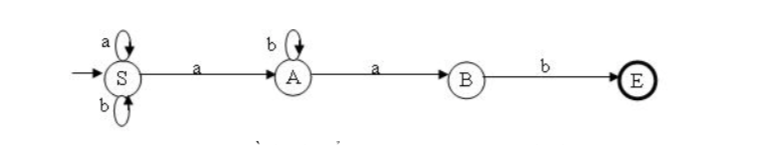
\includegraphics[scale=0.5]{3_21.png}
\caption{ \textit{Đồ thị chuyển của otomat A trong thí dụ 3.2}}
\end{figure}
Theo định lý trên, otomat A đoán nhận ngôn ngữ chính quy L, thật vậy ta có:\\
$T(A) = \{wab^nab | n \ge 0, w \in \{a, b\}^*\} = L$\\
\textbf{Định lý 3.4} Nếu L là ngôn ngữ được đoán nhận bởi một otomat hữu hạn đơn định thì L là một ngôn ngữ chính quy.\\
Chứng minh: Giả sử $L = T(M), với M = <Q, \sum, \delta, q_0, F>$ là một otomat hữu hạn đơn định. Xét
văn phạm $G = <\sum, Q, q_0, P>$, trong đó $P = \{q \to ap | \delta(q, a) = p\} \cup \{q \to a | \delta(q, a) = p \to F\}$. Khi
đó G là một văn phạm chính quy.\\
\hspace{10mm}$\bullet$ Ta chứng minh L(G) = L, với giả thiết $\varepsilon \not \in L.$\\
1/. Lấy $w = a_1a_2...a_n \in L(G), w \ne \varepsilon$, trong G tồn tại suy dẫn $q_0 \models w hay q_0 \vdash a_1q_1 \vdash a_1a_2q_2 \vdash$
$... \vdash a_1a_2...a_{n-1}q_{n-1} \vdash a_1...a_{n-1}a_n = w.$\\
Do đó $q_0 \to a_1q_1, q_1 \to a_2q_2,..., q_{n-1} \to a_{n-1}q_{n-1}, q_{n-1} \to a_n \in P$ hay ta có\\
$p1 = \delta(q_0, a_1), p_2 = \delta(q_1, a_2),..., q_{n-1} = \delta(q_{n-2}, a_{n-1}), q_n \in F$\\
tức là $\delta(q0, w) = q_n \in F$ hay $w  \in T(A) = L$\\
2/. Lấy $w = a_1a_2...a_n \in L, w \ne \varepsilon$, khi đó tồn tại dãy trạng thái $q_1, q_2,..., q_n$ sao cho $\delta(q_0, a_1)$ = p1, $\delta q_1, a_2) = q_2,..., \delta(q_{n-2}, a_{n-1}) = q_{n-1}, \delta(q_{n-1}, a_n) = q_n \in F$. Do đó trong G có các quy tắc $q_0 \to a_1q_1, q_1 \to a_2q_2,..., q_{n-1} \to a_{n-1}q_{n-1}, q_{n-1} \to a_n \in P$, ta có suy dẫn trong $G: q0 \vdash a_1q_1 \vdash a_1a_2q_2 \vdash
...\vdash a_1a_2...a_{n-1}q_{n-1}\vdash a_1...a_{n-1}a_n = w hay w \in L(G).$\\
\hspace{10mm}$\bullet$ Trong trường hợp $\varepsilon \in$ L, ta xây dựng G' tương đương với G trong đó ký hiệu xuất
phát không xuất hiện trong bất kỳ vế phải của quy tắc nào, đồng thời thêm vào G' quy tắc
$q_0 \to \varepsilon$ để nhận được văn phạm chính quy G’ sao cho $L(G') = L(G) \cup \{\varepsilon\}$. Vậy ta luôn có
L(G) = L. Vậy định lý được chứng minh.\\
\hspace{10mm} \textbf{Thí dụ 3.3} Cho otomat hữu hạn đơn định $A = <\{q_0, q_1, q_2\}, \{0, 1\}, \delta, q_0, \{q2\}>$, trong
đó $\delta(q_0, 0) = q_1, \delta(q_1, 0) = q_2, \delta(q_1, 1) = q_0, \delta(q_2, 1) = q_0$. Đồ thị chuyển của A là:\\
\begin{figure}[ht]

\includegraphics[scale=0.5]{3_22.png}
\caption{ \textit{Đồ thị chuyển của otomat A trong thí dụ 3.3}}
\end{figure}
Dễ thấy rằng T(A) = $\{w00 | w \in \{01, 001\}^*\}$ là ngôn ngữ chính quy.\\
\textbf{Kết luận} Từ các định lý trên ta có kết luận về sự liên hệ giữa otomat hữu hạn và ngôn ngữ chính quy như sau:\\
1/. Gọi D là lớp các ngôn ngữ được đoán nhận bởi otomat hữu hạn đơn định, N là lớp các
ngôn ngữ được đoán nhận bởi otomat hữu hạn không đơn định và R là lớp các ngôn ngữ
chính quy.
\hspace{10mm}Định lý 2.1 cho biết D = N.\\
\hspace{10mm}Định lý 3.3 cho biết $R \subset N$.\\
\hspace{10mm}Định lý 3.4 cho biết $D \subset R$\\
\hspace{10mm}Vậy D = N = R.\\
2/. Ngôn ngữ L là chính quy khi và chỉ khi:\\
\hspace{10mm}a/. Tồn tại một biểu thúc chính quy biểu diễn L,\\
\hspace{10mm}b/. Tồn tại một văn phạm chính quy sinh ngôn ngữ L,\\
\hspace{10mm}c/. Tồn tại một otomat hữu hạn đoán nhận L\\
\textbf{Thí dụ 3.4} Với ngôn ngữ chính quy L = $\{01^n, 021 | n \ge 1\}$, ta có:\\
\hspace{10mm}$\bullet$ Biểu thức chính quy biểu diễn L (xem thí dụ 3.2) là:
r = 01*1+021\\
\hspace{10mm}$\bullet$ Văn phạm chính quy sinh ngôn ngữ L:
$G = <\{0, 1, 2\}, \{S, A, B, C\}, S, \{S \to 0A, A \to 1A, A \to 1, S \to 0B, B \to 2C, C \to 1\}>$\\
\hspace{10mm}$\bullet$ Otomat hữu hạn A đoán nhận L có đồ thị chuyển là:\\
\begin{figure}[ht]

\includegraphics[scale=0.5]{3_23.png}
\caption{ \textit{Đồ thị chuyển của otomat A trong thí dụ 3.4}}
\end{figure}
\section{Điều kiện cần của ngôn ngữ chính quy}
\hspace{10mm} Khi một ngôn ngữ được đoán nhận bởi otomat hữu hạn, hoặc được sinh bởi một văn
phạm chính quy, hoặc được xác định bởi một biểu thức chính quy thì nó là ngôn ngữ chính
quy. Như vậy việc chứng minh một ngôn ngữ là chính quy là khá dễ dàng bằng cách chỉ ra
rằng nó được xác định bằng một trong những cách trên. Tuy nhiên, để khẳng định một ngôn
ngữ L không phải là ngôn ngữ chính quy thì lại không hề đơn giản. Dù ta không xây dựng
được otomat hữu hạn, văn phạm chính quy hay biểu thức chính quy để xác định L, nhưng ta
vẫn không thể kết luận được ngôn ngữ này không phải là ngôn ngữ chính quy, bởi vì ta không
thể khẳng định được rằng không tồn tại những văn phạm chính quy hay những otomat hữu
hạn sinh ra L. Như vậy, cần có một tiêu chuẩn để căn cứ vào đó có thể kết luận một ngôn ngữ
không phải là ngôn ngữ chính quy, tiêu chuẩn đó là điều kiện cần của ngôn ngữ chính quy.

\textbf{4.1 Otomat tối tiểu} Cùng một ngôn ngữ chính quy L, có thể có nhiều otomat hữu hạn đoán nhận nó. Tuy
nhiên, trong số đó, trước hết chúng ta quan tâm đến các otomat có số trạng thái ít nhất cùng
đoán nhận ngôn ngữ L.\\
\textbf{Định nghĩa 4.1} Otomat có số trạng thái ít nhất trong các otomat hữu hạn cùng đoán nhận
ngôn ngữ L được gọi là otomat tối tiểu của ngôn ngữ L.\\
\textbf{Nhận xét:} Dễ thấy rằng với mỗi ngôn ngữ L, otomat tối tiểu của nó có thể không duy nhất.\\
\textbf{Thí dụ 4.1} Giả sử ta có otomat M = $<Q, \{a, b\}, \delta, t_0, F>$, với\\
+ $Q = \{t_0, t_1, t_2, t_3\}, với t_0 = \{q_0\}, t_1 = \{q_1\}, t_2 = \{q_0, q_1\}, t 3 = \O.$\\
+ $\delta(t_0, a) = t_0, \delta(t_0, b) = t_2, \delta(t_1, a) = t_2, \delta(t_1, b) = t3, \delta(t_2, a) = t_2, \delta(t_2, b) = t_2, \delta(t_3, a) = t_3, \delta'(t_3,
b) = t_3.$\\
+ $F = \{t_1, t_2\}.$\\
otomat M là đơn định, có 4 trạng thái và có đồ thị chuyển như sau:\\
\begin{figure}[ht]

\includegraphics[scale=0.5]{3_24.png}
\caption{ \textit{Đồ thị chuyển của otomat M trong thí dụ 4.1}}
\end{figure}
Dễ thấy rằng otomat M đoán nhận ngôn ngữ:\\
$L = T(M) = \{a^nbw | n \ge 0, w \in \{a, b\}^*\}.$\\
Nhìn vào đồ thị chuyển của M, ta thấy ngay rằng không có đường đi nào từ t0 đến được đỉnh
kết thúc t1, vì vậy otomat M sẽ tương đương với otomat M’ có đồ thị chuyển như sau:\\
\begin{figure}[ht]

\includegraphics[scale=0.5]{3_25.png}
\caption{ \textit{Đồ thị chuyển của otomat M trong thí dụ 4.1}}
\end{figure}
Rõ ràng là otomat M’ cũng đoán nhận ngôn ngữ L = T(M’) = $\{a^nbw | n \ge 0, w \in \{a, b\}^*\}, M'$ chỉ
có hai trạng thái và là otomat tối tiểu của ngôn ngữ L = $\{a^nbw | n \ge 0, w \in \{a, b\}^*\}$.\\
\textbf{4.2 Điều kiện cần của ngôn ngữ chính quy}\\
\textbf{Định lý 4.1} Nếu L là ngôn ngữ chính quy thì tồn tại số nguyên dương n sao cho với mọi $w$
$\in$ L mà $|w | \ge n$ đều có thể phân tích được dưới dạng $w = uvw$, (với $|v| \ge 1$ hay $v \ne \varepsilon$) mà với
mọi chỉ số $i = 0, 1. 2,... $ta có $uv^iw \in L$\\
\textit{Chứng minh: }Vì L là một ngôn ngữ chính quy, khi đó tồn tại một otomat hữu hạn đoán nhận
nó. Giả sử L = T(A) , với A = $<Q, \sum, \delta, q_0, F>$ là một otomat tối tiểu có n trạng thái, tức là |Q|
= n. Ta chứng minh n là số tự nhiên cần tìm.\\
Giả sử $ww = a_1a_2...a_m \in L $với m $\ge$ n. Khi đó ta có $\delta(q_0, ww) \in F$, tức là $\exists q_0, q_1..., q_m \in Q$ sao
cho $(q_{i-1}, a_i) = q_i, 1 \le i \le m$ và $q_m \in F$. Do $m \ge n$ nên trong dãy $q_0, q_1,..., q_m$ có ít nhất hai
trạng thái trùng nhau, giả sử đó là $q_i = q_k, i < k \le n$, (với k là số nhỏ nhất mà ta có $q_i = q_k$)\\
\hspace{10mm} Đặt $u = a_1...a_i, v = a_{i+1}...a_k, w = a_{k+1}...a_m$. Ta có $w = uvw, |v| = |a_{i+1}...a_k| \ge 1 (do i<k).$\\
Ngoài ra ta có:\hspace{10mm} $\delta(q_0, u) = q_i = q_k = \delta(q_0, uv),$\\
theo bổ đề 1.1:\hspace{10mm} $\delta(q_0, u) = \delta(q_0, uv) = \delta(\delta(q_0, u), v) = \delta(\delta(q_0, uv), v) = \delta(q_0, uv^2),$\\
Tương tự, ta có:\hspace{10mm} $\delta(q_0, u) = \delta(q_0, uv^2) = \delta(\delta(q_0, u), v^2) = \delta(\delta(q_0, uv), v^2) = \delta(q_0, uv^3),$\\
tiếp tục ta được:\hspace{10mm} $\delta(q_0, u) = \delta(q_0, uv^i), \forall i \in N.$\\
Cuối cùng ta có:\hspace{10mm} $\delta(q_0, uv^iw) = \delta(\delta(q_0, uv^i), w) = \delta(\delta(q_0, uv), w) = \delta(q_0, uvw) \in F$.

Vậy $uv^iw \in L, \forall i = 0, 1, 2,...$\\
Định lý được chứng minh.\\
\textbf{Hệ quả 4.1}  Cho A là otomat hữu hạn đơn định có n trạng thái và L là ngôn ngữ được đoán
nhận bởi A. Khi đó $L \ne \O$ khi và chỉ khi $\exists w \in L$ sao $|w| < n.$\\
\textit{Chứng minh:} Điều kiện đủ là hiển nhiên. Bây giờ cho $L \ne \O$. Giả sử mọi từ trong L đều có độ
dài $\ge$ n. Gọi $\alpha$ là từ có độ dài nhỏ nhất trong L, mà |$\alpha$| $\ge$ n. Theo định lý 4.1, ta có $\alpha = uvw,$
trong đó $|v| \ge 1$ và với mọi $i = 0, 1, 2,...$ ta có $uv^iw \in L$. Với i = 0, $uw \in L$ mà $|uw| < |\alpha|$ . Điều
này mâu thuẫn với tính nhỏ nhất của $|\alpha|$. Vậy tồn tại $w \in L$ sao cho $|w| < n.$\\
\textbf{Hệ quả 4.2} Tồn tại một ngôn ngữ phi ngữ cảnh mà không được đoán nhận bởi bất kỳ một
otomat hữu hạn đơn định nào.\\
\textit{Chứng minh:} Xét ngôn ngữ $L = \{a^nb^n | n \ge 1\}$ trên bảng chữ $\sum = \{a, b\}$. Ta có L = L(G), trong
đó $G = <\sum, \{S\}, S, \{S \to aSb, S \to ab\}>$ là văn phạm phi ngữ cảnh. Giả sử L = T(A) với A =
$<Q, \sum, \delta, q_0, F>$ là một otomat hữu hạn đơn định. Với n đủ lớn, $\alpha = a^nb^n$ có |$\alpha$| $\ge$ |Q|. Theo
định lý 1.1, ta có thể biểu diễn $a^nb^n = uvw$, trong đó |v| $\ge$ 1, $uv^iw \in L, \exists i = 0, 1, 2,...$ Ta hãy tập
trung phân tích t ừ v và $v^i$:
\hspace{10mm} - Nếu v chỉ chứa a ($|v|_a >0$ và $|v|_b$ = 0) thì với i đủ lớn |$uv^i w |_a > | uv^i w|_b.$\\
\hspace{10mm} - Nếu v chỉ chứa b ($|v|_b >0$ và $|v|_a = 0$) thì với i đủ lớn $| uv^i w |_b > |uv^i w|_a$\\
\hspace{10mm} - Nếu $|v|_a >0$ và $|v|_b > 0 $ thì với i = 2 ta có v = $(ab)^2 = abab$, tức là a và b xen kẽ nhau
trong $uv^iw$, khi đó $uv^iw$ không thể có dạng $a^nb^n$.\\
Cả ba trường hợp đều mâu thuẫn với $uv^iw \in L$. Vậy không tồn tại một otomat hữu hạn đơn
định nào đoán nhận L, tức là L không phải là một ngôn ngữ chính quy.\\
Hệ quả này là một ứng dụng điều kiện cần của ngôn ngữ chính quy, để chứng minh
một ngôn ngữ không phải là chính quy nếu nó không thỏa mãn điều kiện cần này.\\
Hệ quả trên cho thấy rằng tồn tại một ngôn ngữ phi ngữ cảnh mà không phải là ngôn
ngữ chính quy, tức là lớp các ngôn ngữ chính quy là tập con thực sự của lớp các ngôn ngữ phi
ngữ cảnh.\\
\textbf{Bài tập chương 2}\\
1. Hãy xây dựng các otomat hữu hạn có đồ thị chuyển sau và xác định các ngôn ngữ được
đoán nhận bởi chúng.\\
\begin{figure}[ht]
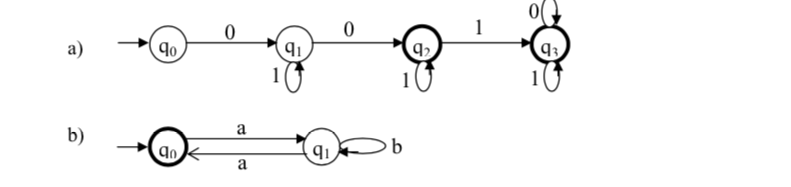
\includegraphics[scale=0.5]{3_26.png}
\end{figure}
2. Hãy xây dựng các otomat hữu hạn đơn định đoán nhận các ngôn ngữ sau:\\
\hspace{10mm} a) L = $\{a^nb^m | n \ge 1, m \ge 1\}.$\\
\hspace{10mm} b) L = $\{(01)^n, (010)^n | n \ge 0\}.$\\
\hspace{10mm} c) L = $\{(aab)^n(baa)^m | n \ge 1, m \ge 1\}.$\\
3. Hãy xây dựng các otomat hữu hạn đơn định đoán nhận các ngôn ngữ sau:\\
\hspace{10mm} a) L1 = $\{w \in \{0, 1\}^* | w$ bắt đầu đúng 3 chữ số 0$\}$.\\
\hspace{10mm} b) L2 = $\{ w \in \{0, 1\}^* | w$ không bắt đầu bởi hai chữ số 1 liên tiếp$\}$.\\
4. Hãy xây dựng các otomat hữu hạn đoán nhận các ngôn ngữ phần bù của các ngôn ngữ L1
và L2 trong bài tập 3.\\
Chú ý : Otomat huu han đơn định và đầy đủ thì phần bù của nó la otomat đổi két thành không
kết và ngược lại.\\
5. Hãy xây dựng các otomat hữu hạn không đơn định đoán nhận các ngôn ngữ sau:\\
\hspace{10mm} a) L = $\{w_1abaw_2 | w_1, w_2 \in \{a, b\}^*\}.$\\
\hspace{10mm} b) L = $\{w \in \{0, 1\}^* | w$ bắt đầu bằng luỹ thừa dương của 101$\}$.
\hspace{10mm} c) L = $\{(1111)^nw | w \in \{0, 1\}^*, n \ge 0\}.$\\
6. Hãy thành lập các văn phạm chính quy sinh ra các ngôn ngữ mà được đoán nhận bởi các
otomat hữu hạn không đơn định sau:\\
\hspace{10mm} a) A = $<\{q_0, q_1, q_2, q_3, q_4\}, \{a, b\}, \delta, q_0, \{q_2, q_4\}>,$ trong đó:\\
$\delta(q_0, a) = \{q_0, q_1\}, \delta(q_0, b) = \{q_0, q_1\}, \delta(q_1, a) = \O, \delta(q_1, b) = \{q_2\}, \delta(q_2, a) = \{q2\}, \delta(q_2, b) =
\{q_2\}, \delta(q_3, a) = \{q_4\}, \delta(q_3, b) = \O, \delta(q_4, a) = \{q_4\}, \delta(q_4, b) = \{q_4\}.$\\
\hspace{10mm} b) $A = <\{q_0, q_1\}, \{0, 1\}, \delta, q_0, \{q_1\}>$, trong đó:\\
$\delta(q_0, 0) = \{q_0, q_1\}, \delta(q_0, 1) = \{q_1\}, \delta(q_1, 0) = \O, \delta(q_1, 1) = \{q_0, q_1\}.$\\
7. Hãy xây dựng các otomat hữu hạn đơn định đoán nhận các ngôn ngữ mà được sinh bởi các
văn phạm chính quy sau:\\
\hspace{10mm} a) $G = <\{a, b, c\}, \{S, A, B, C, D\}, S, \{S \to aB, S \to aC, B \to aA, C \to bD, D \to bC, D \to bA, A \to cA, A \to c\}>.$\\
b) $G = <\{0, 1\}, \{S, A, B, C, D, E\}, S,\{S \to \varepsilon, S \to 1A, B \to 0C, B \to 0D, A \to 1B, B \to 1D,
D \to 0E, C \to 1B, C \to 0A, E \to 1A, D \to 1E, E \to 0B, A \to 0D, E \to 1, C \to 1\}>.$\\
8. Hãy xây dựng các otomat hữu hạn đơn định đoán nhận các ngôn ngữ được biểu diễn bởi
các biểu thức chính quy sau:\\
\hspace{10mm} a) $bba(a+b)^*$. \\
\hspace{10mm} b) $(a+b)^*bab.$ \\
\hspace{10mm} c) $(bb+a)^*$ \\
\hspace{10mm} d) $(aa+b)^*.$ \\
\hspace{10mm} e) $(bb+a)^*(aa+b)^*.$ \\
9. Cho ôtomat $A = (S, \sum , s_1, \delta, F)$, với tập trạng thái S = $\{s_1, s_2, s_3, s_4\}$, bảng chữ cái $\sum = \{ a,
b\}$, F = $\{s_4\}$, và hàm chuyển trạng thái cho bởi bảng sau:\\
\begin{figure}[ht]
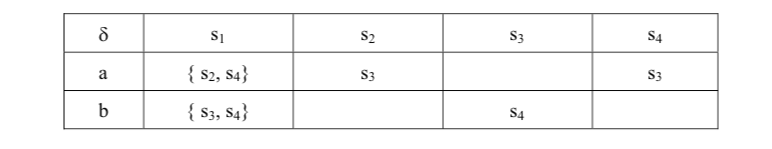
\includegraphics[scale=0.5]{3_27.png}
\end{figure}

\hspace{10mm} a. Viết đồ thị chuyển của ôtomat A.\\

\hspace{10mm} b. Tìm otomat M đơn định và đầy đủ tương đương với otomat A\\
\hspace{10mm} c. Viết đồ thị chuyển của ôtomat M\\
10. Cho otomat$ A = (S, \sum , s_1, \delta, F)$, với tập trạng thái $S = \{s_1, s_2, s_3\}, \sum = \{ a, b, c\}, F = \{s_3\},$
và hàm chuyển trạng thái cho bởi bảng sau:\\
\begin{figure}[ht]
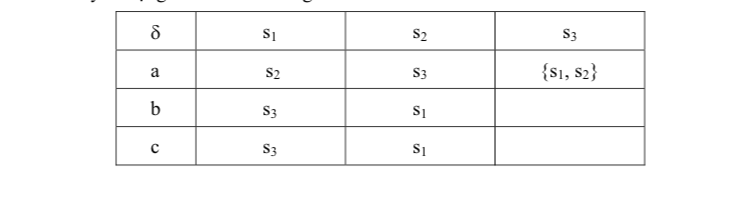
\includegraphics[scale=0.5]{3_28.png}
\end{figure}
\hspace{10mm} a. Viết đồ thị chuyển của otomat A.\\
\hspace{10mm} b. Tìm otomat $M = (Q, \sum , q_1, f, P$ ),đơn định và đầu đủ, tương đương với otomat A\\
\hspace{10mm} c. Viết đồ thị chuyển của otomat M.






\end{flushleft}






\chapter{KIỂM ĐỊNH MÃ VÀ MÃ MỞ RỘNG}

\begin{flushleft}
Chương này, ta đề xuất các thuật toán mới kiểm định mã, $w$-mã, $w$-mã và Z-mã. Trong mỗi mục, từ \hyperlink{42}{\textcolor{blue}{2.1}} đến mục \hyperlink{page.52}{\textcolor{blue}{2.3}}, từng thuật toán được trình bày theo thứ tự chúng được thiết lập. Một tiêu chuẩn mới kiểm định mã mở rộng từ tiêu chuẩn kinh điển Sardinas-Patterson và thuật toán hiệu quả kiểm định mã được giới thiệu trong hai mục nhỏ, mục \hyperlink{page.42}{\textcolor{blue}{2.1.1}} và mục \hyperlink{page.32}{\textcolor{blue}{2.1.2}} của mục \hyperlink{page.42}{\textcolor{blue}{2.1}}. Trước hết trong mục \hyperlink{page.42}{\textcolor{blue}{2.1.1}}, ta xem xét thủ tục trên ngôn ngữ để nhận biết phương pháp của thuật toán. Tiếp theo, trong mục \hyperlink{page.42}{\textcolor{blue}{2.1.2}}, thuật toán dựa trên các vị nhóm hữu hạn được thiết lập với giả thiết đầu vào là một ngôn ngữ chính quy $X$ chơ bởi một bộ ba ($\varphi, M, B$), với $\varphi : A^* \to M$ là một đồng cấu vị nhóm thoả $X, M$ là một vị nhóm hữu hạn, $B \subseteq M, X = \varphi^{-1} (B)$ và $n = Card(M)$. Phương pháp của tiêu chuẩn mới kiểm định mã mở rộng cho $\Diamond$-mã và thuật toán kiểm định được trình bày trong mục \hyperlink{page.44}{\textcolor{blue}{2.1.3}}. \\
\hspace{10mm}Trong hai mục đầu của mục \hyperlink{page.46}{\textcolor{blue}{2.2}}, ta đưa vào các tiêu chuẩn và thuật toán kiểm định kiểu Sardinas-Patterson thiết lập mã cho $w$-mã. Kết quả chính của phần này là một thuật toán hiệu quả dựa trên đồ thị có hướng với cung cấp có gán màu xem như một hệ quả của thuật toán dựa trên các vị nhóm hữu hạn. Các tiêu chuẩn và thuật toán kiểm định kiểu Sardinas-Patterson thiết lập cho Z-mã được trình bày theo các tương tự trong mục \hyperlink{page.52}{\textcolor{blue}{2.3}}.\\
\hspace{10mm}Một số kết quả chính của chương trình được công bố trong các bài báo số 3, 4, 5-9, 13 (xem Danh mục các công trình đã công bố của luân án).\\
\section{Thuật toán kiểm định mã và $\Diamond$-mã}
\subsection{Tiêu chuẩn Sardinas-Patterson mở rộng}
Dụa trên Nhận xét \hyperlink{page.18}{\textcolor{blue}{1.4}}, trong mục này ta đề xuất một thủ tục mới để kiểm tra một ngôn ngữu chính quy $X \subseteq A^+$ cho trước có là mã không. Bằng phương pháp tổ hợp mới, ta tính toán các tập phần tư $V_i$ kết hợp với $X$ dưới dạng công thức để quy như sau:
\end{flushleft}
$V_i = X^{-1}X - \{ \varepsilon \}$ \begin{flushright}
        (2.1)
\end{flushright}
$V_{i+1} = V_i^{-1}X \cup X^{-1}V_i \cup V_i$, $i \ge 1$
\begin{flushleft}
\hspace{10mm}Phương pháp của thủ tục được minh hoạ trong Hình \hyperlink{page.43}{\textcolor{blue}{2.1}}. Các tập $V_i (i \ge 1)$ nhận được từ thủ tục theo phương pháp tổ hợp mới sẽ thoả tính chất bao hàm $V_i \subseteq V_{i+1}, \forall i$.
\end{flushleft}
\begin{figure}[ht]
    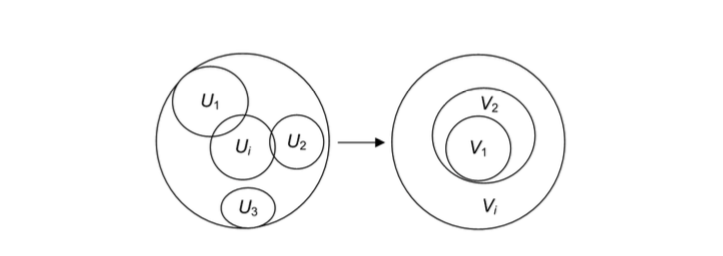
\includegraphics[scale=0.5]{2_1.png}
    \caption{ \textit{Một hướng cải tiến tiêu chuẩn kiểm định mã Sardinas-Patterson} }
\end{figure}
\begin{flushleft}
\hspace{10mm}Tính đúng đắn của thủ tục dựa trên Định lý \hyperlink{page.43}{\textcolor{blue}{2.1}} và các bổ đề sau đây.\\
\textbf{Bổ đề 2.1}      \textit{Cho $X \subseteq A^+$ và $V_i(i \ge 1)$ được định nghĩa theo công thức \hyperlink{page.42}{\textcolor{blue}{2.1}}Khi đó, với $z \in A^*$ tuỳ ý, $k \ge 1$, nếu $z \in V_k$ thì tồn tại $n,m \ge 1, x_1,x_2,...,x_n, y_1, y_2,...,y_m \in X$ sao cho}.
\end{flushleft}
$x_1x_2...x_n z = y_1y_2...y_m$ với $x_1 \ne y_1$.
\begin{flushleft}
\textit{Chứng minh}. Ta chứng minh quy nạp theo $k$ khẳng định trên.\\
\hspace{10mm} Với $k = 1$, giả sử $z \in V_1$ ta phải chứng minh tồn tại $n,m \ge 1, x_1, x_2, ..., x_n, y_1, y_2, ...,y_m \in X$, sao cho $x_1x_2...x_nz = y_1y_2...y_m$ với $x_1 \ne y_1$.\\
\hspace{10mm}Từ định nghĩa $V_1 = X^{-1}X - \{ \varepsilon \}, z\in V_1$, suy ra $z \in X^{-1}X = \{ \varepsilon \}$, nghĩa là tồn tại $x_1, y_1 \in X$ sao cho $x_1z \ y_1$. vì $\varepsilon \not\in V_1$ suy ra $x_1 \ne y_1$. \\
\hspace{10mm}Vậy, điều khẳng định đúng với k = 1.\\
\hspace{10mm}Giả sử điều khẳng định đã đúng với $k > 1$, ta chứng minh nó cũng đúng với trường hợp $k + 1$.\\
\hspace{10mm}Giả sử $z \in V_{k+1}$, ta phải chứng minh tồn tại $n,m \ge 1, x_1, x_2, ... , x_n, y_1, y_2,...,y_m \in X$ sao cho $x_1x_2...x_n z = y_1y_2...y_m$với $x_1 \ne y_1$.\\
\hspace{10mm}Theo định nghĩa $V_{k+1} = V^{-1}X \cup X^{-1}V_k \cup V_k$. Khi đó, từ $z \in V_{k+1}$, suy ra $z \in V_k$ (trường hợp 1) hoặc $z \in V_k^{-1}X$ (trường hợp 2) hoặc $z \in X^{-1}V_k$ (trường hợp 3). Ta xét các trường hợp sau.\\
\hspace{10mm}Trường hợp 1: $z \in V_k$. Theo giả thiết quy nạp, điều khẳng định đúng.
\hspace{10mm}Trường hợp 2: $z \in V^{-1}X$. Tồn tại $z' \in V_k$, theo giả thiết quy nạp, tồn tại $l,s \ge 1,x_1,x_2,...,x_l, y_1, y_2,...,y_s \in X$ sao cho
\end{flushleft}
$x_1x_2...x_1 z' = y_1y_2...y_s$ với $x_1 \ne y_1$.
\begin{flushleft}
Nhân $z$ vào hai vế của biểu thức trên, ta có
\end{flushleft}
$x_1x_2...x_l z' z = y_1y_2...y_s z$ với $x_1 \ne y_1$.
\begin{flushleft}
Thay $z'z = x$ vào biểu thức trên ta nhận được
\end{flushleft}
$x_1x_2...x_lx = y_1y_2....y_sz$ với $x_1 \ne y_2$ 
\begin{flushleft}
\hspace{10mm}Vậy, điều khẳng định đúng với mọi $k \ge 1$.
\hspace{10mm}Chứng minh được hoàn thành
\textbf{Bổ đề 2.2}     \textit{Cho $X \subseteq A^+ $ và $V_i (i \ge 1)$ được định nghĩa theo công thức (2.1). Nếu có $n,m \ge 1, x_1, x_2,...,x_n, y_1, y_2, ... , y_m \in X$ và $z \in A^*$ tuỳ ý sao cho}
\end{flushleft}
$x_1x_2...x_nz = y_1y_2...y_m$ với $x_1 \ne y_1$ và $|z| \le |y_m|$
\begin{flushleft}
thì tồn tại $k \ge 1 $ sao cho $z \in V_k$.\\
\textit{Chứng minh}. Ta chứng minh quy nạp theo $n + m$ điều khẳng định trên.\\
\hspace{10mm}Với $n+m = 2 (n = 1, m = 1)$, từ dãy $x_1z = y_1$ với $x_1 \ne y_1$ và $|z| \le |y_1|$ ta có $\varepsilon \ne z = x_1^{-1}y_1 \in X^{-1}X = \{ \varepsilon \} = V_1$.\\
\hspace{10mm}Vậy điều khẳng định đúng với n + m = 2.\\
\hspace{10mm}Giả sử điều khẳng định đúng với $n + m -1 \ge 2$, ta chứng minh nó cũng đúng với $n + m$. Từ đẳng thức $x_1x_2...x_nz = y_1y_2...y_m$ với $x_1 \ne y_1$ và $|z| \le |y_m|$, ta phải chứng minh tồn tại $k \ge 1$ sao cho $z \in V_k$.\\
\hspace{10mm}Ta xét ba khả năng sau có thể xảy ra khi so sánh độ dài của $x_nz$ và từ $y_m$.\\
\hspace{10mm}Trường hợp 1: $|x_nz| < |y_m|$. Theo giả thiết quy nạp, tồn tại $k \ge 1$ sao cho $x_nz \in V_k$.
Khi đó, $x_n^{-1}V_k = z \in V_{k+1}$.\\
\hspace{10mm}Trường hợp 2: $x_nz = y_m$. Ta có $x_n^{-1}y_m = z$. Ta có $x_n^{-1}y_m = z$. Nếu $z \ne \varepsilon$ thì $z \in X^{-1}X = \{ \varepsilon \} = V_1$. Ngược lại, nếu $z = \varepsilon$ thì $\varepsilon \in V_k$ với $k > 1$ nào đó.\\
\hspace{10mm} Thật vậy, theo giả thiết ta có 
\end{flushleft}
$x_1x_2...x_nz = y_1y_2...y_m$ với $x_1 \ne y_1$ và $|z| \le |y_m|$.
\begin{flushleft}
Vì $x_nz = y_m$, ta suy ra
\end{flushleft} 
$x_1x_2...x_{n-1} = y_1y_2...y_{m-1}$ với $x_1 \ne y_1$,
\begin{flushleft}
hoặc tương đương,
\end{flushleft}
$x_1x_2...x_{n-1}\varepsilon = y_1y_2...y_{m-1}$ với $x_1 \ne y_1$,
\begin{flushleft}
Theo giả thiết quy nạp, $\varepsilon \in V_k$ với $k \ge 1$ nào đó.\\
\hspace{10mm}Trường hợp 3: $|x_nz| > |y_m|$. Theo giả thiết $|z| < |y_m|$, suy ra tồn tại $u \in A^+$ sao cho $y_m \ uz$. Từ $|x_nz| > |y_m|$ và $y_m = uz$, suy ra tồn tại $u' \in A^+$, $y_s \in X$, $1 \le s \le m - 1$, $|u'| \le |y_s|$ sao cho $x_n = u'y_{s+1}y_{s+1}...y_{m-1}u$.
\hspace{10mm}Hơn nữa theo giả thiết, ta có 
\end{flushleft}
$x_1x_2...x_{n-1} = y_1y_2...y_{m-1}$ với $x_1 \ne y_1$ và $|z| \le |y_m|$.
\begin{flushleft}
Thay $y_m = uz$ và $x_n = u'y_{s+1}y_{s+2}...y_{m-1}u$ vào biểu thức trên ta nhận được 
\end{flushleft}
$x_1x_2...x_{n-1}u' = y_1y_2...y_s$ với $x_1 \ne y_1$ và $|u'| \le |y_s|$.
\begin{flushleft}
Theo giả thiết quy nạp, ta suy ra $u' \in V_k$ với $k \ge 1$ nào đó. Ta có 
\end{flushleft}
$u'^{-1}x_n = y_{s+1}y_{s+2}...y_{m-1}u \in V_{k+1} = V_k^{-1}X$ \\
$\Rightarrow y_{s+1}^{-1}V_{k+1} = y_{s+2}...y_{m-1}u \in V_{k+2}$\\
...\\
$y_{m-1}^{-1}V_{k+m-1} = u \in V_{k+m} \Rightarrow u^{-1}y_m = z \in V_{k+m+1}$.
\begin{flushleft}
Vậy, điều khẳng đúng với mọi $n+m \le 2$.\\
Chứng minh được hoàn thành.\\
\hspace{10mm}Trong định lý \hyperlink{page.43}{\textcolor{blue}{2.1}} sau đây, ta thiết lập kết quả chính của mục này nhằm cung cấp một tiêu chuẩn mới kiểm định mã mà từ nay về sau trong luận án, ta sẽ gọi là tiêu chuẩn Sardinas-Patterson mở rộng.\\
\textbf{Định lý 2.1}    \textit{Cho $X \subseteq A^+$ và $V_i(i \ge 1)$ sao cho $\varepsilon \in V_i$}. Khi đó, theo bổ đề \hyperlink{page.43}{\textcolor{blue}{2.1}} , tồn tại $n,m, \ge 1, x_1, x_2,..., x_n, y_1, y_2,...,y_m \in X$ sao cho
\end{flushleft}
$x_1x_2...x_{n-1}\varepsilon = y_1y_2...y_{m-1}$ với $x_1 \ne y_1$,
\begin{flushleft}
hoặc tương đương,
\end{flushleft}
$x_1x_2...x_{n-1} = y_1y_2...y_{m-1}$ với $x_1 \ne y_1$,
\begin{flushleft}
Đây là hai $X$-phân tích khác nhau của một từ $w \in A^*$. Suy ra X không là mã, mâu thuẫn.

% \textit{Chiều ngược}. Nếu $\varepsilon V_i$ với mọi $i \le 1$ thì X là mã.
\hspace{10mm}Phản chứng, giả sử X không là mã. Khi đó, tồn tại $w \in A^*$ có hai phân tích khác nhau, 
\end{flushleft}
$w = x_1x_2...x_n = y_1y_2...y_m$
\begin{flushleft}
với $x_1 \ne y_1, x_i, y_j \in X$, $i = 1,...,n$, $j = 1,...,m$, hoặc tương đương,
\end{flushleft}
$w = x_1x_2...x_n\varepsilon = y_1y_2...y_m$ với $x_1 \ne y_1$
\begin{flushleft}
Theo bổ đề \hyperlink{page.43}{\textcolor{blue}{2.2}}, tồn tại $i \ge i$ sao cho $\varepsilon \in V_i$, mâu thuẫn.
\hspace{10mm}Chứng minh được hoàn thành.
\hspace{10mm}Từ định lý trên, ta nhận được các hệ quả sau đây
\textbf{Hệ quả 2.1}     \textit{Cho $X \subseteq A^+$}

\end{flushleft}



\chapter{Phương pháp phân rã Dantzig-Wolfe giải bài toán kích thước lớn}
%%%%%%%%%%%%%%%%%%%%%%%%%%%%%%%%%%%%%%%%%%

Phương pháp phân rã Dantzig - Wofle là sự kết hợp giữa ý tưởng về việc giải quyết một bài toán QHTT tổng quát do Philip Wolfe đề xuất và phương pháp phân rã của Dantzig. Do vậy, để xem xét tận gốc của vấn đề, trước hết cần trình bày lại bài toán QHTT tổng quát của Wolfe.
%%%%%%%%%%%%%%%%%%%%%%%%%%%%%%%%%%%%%%%%%%
%+ Bai 2.1. Bai toan QHTT Wolfe tong quat
\section{Bài toán quy hoạch tuyến tính Wolfe tổng quát}

%+ 2.1.1. Phat bieu bai toan
\subsection{Phát biểu bài toán và các tính chất}
Xuất phát từ những bài toán ứng dụng thực tế, các hệ số $A, b$ và $c$ của bài toán QHTT \eqref{eq.2.1.1} thường thay đổi trong một tập nào đó. Điều này cho phép việc ứng dụng vào thực tế trở nên mềm dẻo hơn, phù hợp với ứng dụng thực tế hơn. Khi các hệ số $A, b, c$ thay đổi trong các tập lồi, bài toán này trở thành bài toán QHTT tổng quát được Philip Wolfe đề xuất. 

Bài toán QHTT Wolfe tổng quát được phát biểu như sau:
\begin{align}\label{eq.2.1.1}
&\min\set{f(x) = c^Tx}\\
&\text{thỏa mãn } D := \begin{cases}
Ax=b\\
x\geq 0\\
\end{cases}\notag
\end{align}
trong đó các hệ số $\binom{c_j}{A_j}\in C_j$ với mọi $j=1,\dots, n$. Ở đây, $C_j$ là các tập lồi nào đó trong $\R^{m+1}$ và $A_j$ là véc tơ cột thứ $j$ của ma trận $A$. Tổng quát hơn, người ta cũng có thể xem xét bài toán (\ref{eq.2.1.1}) với hệ số $b_i$ thay đổi, tức $b\in C_b$ nào đó với $C_b$ là tập lồi trong $\R^m$.

Vì các véc tơ $\binom{c_j}{A_j}$ chọn tùy ý trong các tập $C_j$, nên theo định lý biểu diễn tập lồi, với mỗi $j$, véc tơ $\binom{c_j}{A_j}$ có thể biểu diễn qua tập đỉnh và tập hướng cực biên của $C_j$. Trước hết ta sẽ chứng minh một định lý tổng quát cho bài toán Wolfe tổng quát.

%+ Dinh ly 2.1.1
\begin{theorem}\label{th.2.1.1}
Bài toán QHTT Wolfe tổng quát \eqref{eq.2.1.1} là tương đương với bài toán QHTT Wolfe tổng quát sau:
\begin{align}\label{eq.2.1.2}
&\min\set{\hat f(x,x^t) := \sum_{j=1}^n(c_jx_j + \sum_{t=1}^{T_j}c^t_jx_j^t)}\\
&\text{thỏa mãn } D := \begin{cases}
\sum_{j=1}^n(a_{ij}x_j + \sum_{t=1}^{T_j}a^t_{ij}x^t_j) = b_i,\\
x_j \geq 0,\quad i=1,\dots, m,\; j=1,\dots, n.
\end{cases}\notag
\end{align}
trong đó $\binom{c_j}{A_j}$ chọn tùy ý trong $C_j$ và $\binom{c^t_j}{A^t_j}$ là $T_j$ các điểm cố định trong $C_j$.
\end{theorem}
Chú ý rằng bài toán \eqref{eq.2.1.2} có số biến nhiều hơn bài toán \eqref{eq.2.1.1}. Do vậy tính tương đương ở đây thể hiện theo nghĩa, tập nghiệm của hai bài toán có thể suy ra nhau và giá trị hàm mục tiêu là bằng nhau.

%+ Chung minh.
\noindent{\it Chứng minh. }
Giả sử $x_j=x^{*}_j$ và $\binom{c_j}{A_j} = \binom{c^{*}_j}{A^{*}_j}$ với $j=1,\dots, n$ là nghiệm tối ưu của bài toán \eqref{eq.2.1.1} với giá trị $f(x^{*}) = f^{*}$ và giả sử $x_j=\hat x_j, x^t_j=\hat x_j^t$ và $\binom{c_j}{A_j} = \binom{\hat c_j}{\hat A_j}, \binom{c^t_j}{A^t_j} = \binom{\hat c^t_j}{\hat A^t_j},$ với $j=1,\dots, n$ là nghiệm tối ưu của bài toán \eqref{eq.2.1.2} với giá trị hàm mục tiêu tối ưu $\hat f(\hat x) = \hat f$.\\
Dễ thấy $x_j=x_j^{*}, x_j^t=0$ là nghiệm chấp nhận của bài toán \eqref{eq.2.1.2} nên ta có $f^{*}\leq \hat f$. 
Mặt khác, nghiệm tối ưu của bài toán \eqref{eq.2.1.2} có thể viết lại như là nghiệm chấp nhận của bài toán \eqref{eq.2.1.1} dưới dạng:
\begin{align*}
&\min\set{\sum_{j=1}^n\bar c_j\bar x_j}\\
&\text{thỏa mãn } \begin{cases}
\sum_{j=1}^n\bar a_{ij}\bar x_j = b_i,\quad i=1,\dots, m,\\
\bar x_j \geq 0, \quad j=1,\dots, n,
\end{cases}
\end{align*}
trong đó
\begin{align*}
&\bar x_j = \hat x_j + \sum_{t=1}^{T_j}\bar x^t_j,\\
&\binom{\bar c_j}{\bar A_j}= \begin{cases}
\binom{\hat c_j}{\hat A_j}\frac{\hat x_j}{\bar x_j} + \binom{\hat c^t_j}{\hat A^t_j}\frac{\bar x^t_j}{\bar x_j} \quad\text{với $\bar x_j\neq 0$},\\
\binom{\hat c_j}{\hat A_j} \quad\text{với $\bar x_j =  0$}.
\end{cases}
\end{align*}
Điều này có nghĩa là $\bar f \leq f^{*}$. Do vậy $\bar f=f^{*}$.
\hfill $\square$
%+ Ket thuc Dinh ly 2.1.1

Bây giờ để đơn giản việc nghiên cứu, ta hạn chế một số các hệ số $\binom{c_j}{A_j}$ thay đổi trong các tập $C_j$ một số các hệ số khác cố định, trong trường hợp này $\abs{C_j} = 1$ (tập hợp chỉ gồm 1 điểm).
Giả sử ta xét bài toán QHTT tổng quát có dạng:
\begin{equation}\label{eq.2.1.3}
 \begin{array}{lllll}
\min\set{ &c^Tx+y_{0,n+1}x_{n+1}&=z}\\
&Ax+y_{\bullet n+1}x_{n+1}&=b,&&\\
&(x,x_{n+1})&=(x_1,x_2,\dots,x_{n+1})\geq0.
\end{array}.
\end{equation}
trong đó $A=(a_{ij})_{m\times n}$ và các hệ số $\binom{y_{0,n+1}}{y_{\bullet n+1}}\in C_{n+1}$ là tập đơn hình có dạng:
\begin{equation}\label{eq.2.1.4}
C_{n+1}=\{y_{i,n+1}| \sum_{i=0}^m\alpha_iy_{i,n+1}=1,y_{i,n+1}\geq0, \textrm{ với }i=0,\dots,m\}
\end{equation}
Khi đó sử dụng định lý biểu diễn tập lồi, ta sẽ biểu diễn mỗi điểm $u\in C_{n+1}$ qua tập đỉnh của nó
\begin{equation}\label{eq.2.1.5}
(u_0, u) = \sum_{i=0}^m\alpha_iy_{i,n+1}.
\end{equation}
Sau đó thay vào bài toán \eqref{eq.2.1.3} ta sẽ thu được một bài toán QHTT với $n+m+1$ biến $x, \alpha_0,\dots, \alpha_m$. 
Khi đó ta có định lý sau:

%+ Dinh ly 2.1.1.
\begin{theorem}\label{eq.2.1.2}
Bài toán QHTT tổng quát dạng (\ref{eq.2.1.3}) là tương đương với bài toán QHTT thông thường
\begin{equation}\label{eq.2.1.5}
\begin{array}{lllll}
\min\set{& c^Tx+u_0&=w}\\
&Ax+u&=b&\\
&\sum_{i=0}^m\alpha_iu_{i,n+1}&=x_{n+1}\\
&x_1,x_2,\dots,x_{n+1}\geq0,& u_0,u_1,\dots,u_m\geq0
\end{array}.
\end{equation}
trong đó $A=(a_{ij})_{m\times n}$ và $u_i=y_{i,n+1}x_{n+1}$ với giả thiết rằng phương án tối ưu cho \eqref{eq.2.1.5} có $x_{n+1}=x^\ast_{n+1}>0$
\end{theorem}

%+ Chung minh.
\begin{proof}
Ta sẽ chứng minh mỗi phương án tối ưu của \eqref{eq.2.1.3} tìm được một phương án tối ưu của \eqref{eq.2.1.5} và ngược lại. 
Trước hết ta sẽ chỉ ra phương án tối ưu của \eqref{eq.2.1.3} là chấp nhận được cho \eqref{eq.2.1.5}. Giả sử $x^{*}$, $y_{i, n+1}^{*}$ và $z^{*}$ là tối ưu cho bài toán \eqref{eq.1.2.3}. Đặt $z=z^\ast$, $x_j=x_j^\ast$, $j=1,\dots,n+1$ với $x_{n+1}^\ast\geq 0$, và $y_{i,n+1}=y_{i,n+1}^\ast$, $i=0,\dots,m$. Khi đó nó là một phương án tối ưu chấp nhận được cho \eqref{eq.2.1.5}. Thật vậy, giá trị $x_j=x_j^\ast$, $j=1,\dots,n+1$ và $u_i=y_{i,n+1}^\ast x_{n+1}^\ast$, $i=0,\dots,m+1$, rõ ràng là chấp nhận được cho \eqref{eq.2.1.3} nghĩa là:
\begin{equation}\label{2.1.5a}
\begin{array}{llllll}
\min\set{&c^Tx^\ast&+y_{0,n+1}^\ast x^\ast_{n+1}&&=w^\ast}\\
&Ax^\ast&&+y_{\bullet,n+1}^\ast x^\ast_{n+1}&=b,\\
&&&\sum_{i=0}^m\alpha_iy^\ast_{i,n+1}x_{n+1}&=x_{n+1}^\ast.
\end{array}
\end{equation}
Do đó ta có $z^\ast\geq w^\ast$. 
Tiếp theo giả sử rằng $w^\ast$ không tối ưu nhưng tồn tại tập các giá trị $w=\overline{w},x_j=\overline{x_j}$ $j=1,\dots,m+1$ và $u_i=\overline{u_i}$, $i=0,\dots,m+1$ tập này là tối ưu chấp nhận được cho \eqref{eq.2.1.5}. Vì $\overline x_{n+1}>0$ theo giả thiết, ta tính $\overline y_{i,n+1}=\overline u_{n+1}/\overline x_{n+1}$ với $i=0,\dots,m$. Phương án $x_j=\overline x_j$, $j=1,\dots,n+1$ với $y_{i,n+1}=\overline y_{i,n+1}$, $i=0,\dots,m$ rõ ràng là chấp nhận được cho \eqref{eq.2.1.3} và vì vậy $\overline{w}\leq \overline{z}$. Do đó phương án tối ưu hai bài toán là tương đương. 
\end{proof}
%+ Ket thuc Dinh ly 2.1.1

Tiếp theo, để minh họa cho phương pháp Wolfe giải bài toán QHTT dạng \eqref{eq.2.1.3}, ta xem xét ví dụ sau:

%+ Vi du 2.1.1
\noindent{\bf Ví dụ 2.1.1. }
Xét bài toán xác định bởi hệ phương trình (\ref{eq.2.1.6})
\begin{equation}\label{eq.2.1.6}
\begin{array}{llllll}
\min&\set{6x_1&+4x_2&+x_3&+y_{04}x_4 & :=z}\\
&x_1&+x_2&-4x_3&+y_{14}x_4&=5\\
&-x_1&+x_2&-x_3&+y_{24}x_4&=1\\
&x_1\geq 0&x_2\geq 0&x_3\geq 0&x_4\geq 0
\end{array}.
\end{equation} 
với các hệ số $y_{\bullet4}=(y_{04},y_{14},y_{24})$ với $y_{i4}\geq0$ không cố định được chọn tùy ý trong đơn hình
\begin{equation}\label{eq.2.1.7}
C_4=\{y_{\bullet4}|\quad 3y_{04}+y_{14}+2y_{24}=2\textrm{ với } y_{i4}\geq 0\quad i=0,1,2\}
\end{equation}
và các hệ số còn lại cố định.

Giả sử ta có một cơ sở xuất phát của các biến $(-z, x_1, x_2)$, phương án cơ sở chấp nhận được cho dưới dạng:
\begin{displaymath}
(-z)=-24,\quad x_1=2,\quad x_2=3,\quad x_3=x_4 = 0.
\end{displaymath}
Bây giờ sử dụng thuật toán đơn hình để kiểm tra xem phương án đã cho có tối ưu không, ta tìm các nhân tử Lagrange, tức các biến đối ngẫu $\pi$ ứng với phương án đã cho bằng việc giải phương trình $B^T\pi = c_B$, tức $\pi = (B^{-1})^Tc_j$ với $B$ là cơ sở ứng với phương án đã cho ở trên. Giải ra ta có $\pi=(5,-1)^T$ và tính các ước lượng $\bar c_3$ và $\bar c_4$ với $\overline{c_j}=c_j-\pi^TA_{\bullet j}$ ta thu được:
$$
\overline{c_3}=18, \;\overline{c_4}=y_{04}-5y_{14}+y_{24}
$$
tron đó $(y_{04},y_{14},y_{24})\in C_4$. 
Theo thuật toán đơn hình, nếu các ước lượng $\bar c_3, \bar c_4 \geq 0$ thì phương án đang xét là tối ưu. Trong trường hợp này vì $\bar c_3=20>0$ nên chỉ còn $c_4$ là phụ thuộc vào tập $C_4$. Để kiểm tra $\bar c_4$, ta tìm giá trị nhỏ nhất của $\bar c_4$ trên tập $C_4$ bằng việc giải bài toán QHTT:
\begin{equation}\label{eq.2.1.8}
\begin{array}{llllll}
\min &y_{04}&-5y_{14}&+y_{24}&=\overline{c_4}\\
&3y_{04}&+y_{14}&+2y_{24}&=2\\
&&y_{i4}\geq0 & i=0,1,2\\
\end{array}.
\end{equation}
Ta thu được $y_{04}=0$, $y_{14}=2$, $y_{24}=0$ và $\overline{c_4}=-10$. Do đó vẫn tồn tại điểm trong $C_4$ sao cho $\bar c_4 < 0$, tức phương án đang xét  
\begin{displaymath}
(-z)=-24,\quad x_1=2,\quad x_2=3,\quad x_3=x_4 = 0.
\end{displaymath}
chưa phải là phương án tối ưu cho bài toán \eqref{eq.2.1.6}.

Để cải thiện phương án của bài toán \eqref{eq.2.1.6}, ta đưa biến $x_4$ vào cơ sở và tìm một biến đưa ra khỏi cơ sở để có cơ sở mới. Trong trường hợp này, theo quy tắc của phương pháp đơn hình, biến $x_1$ sẽ đưa ra khỏi cơ sở, ta có cơ sở mới là $\set{2, 4}$ với giá trị
$$
(-z)=-4,\quad x_2=1,\quad x_4=2,\quad x_1=x_3=0
$$
Tuy nhiên để bảo toàn biến $y_{i4}$ thu được ở bước trước của thuật toán, thay vì xem xét bài toán \eqref{eq.2.1.6}, theo Định lý \ref{th.2.1.1}, ta xem xét bài toán tương đương với nó có dạng:

\begin{equation}\label{eq.2.1.9}
\begin{array}{lllllll}
&6x_1&+4x_2&+x_3&+0x^{(1)}_4&+y_{04}x_4&=z(\min)\\
&x_1&+x_2&-4x_3&+2x^{(1)}_4&+y_{14}x_4&=5\\
&-x_1&+x_2&-x_3&+0x_4&+y_{24}x_4&=1\\
&x_1\geq 0,&x_2\geq 0,&x_3\geq 0,&x_4\geq 0,&x^{(1)}_4\geq 0
\end{array}.
\end{equation} 
ở đây $y_{\bullet 4}\in C_4$.\\
Như ở trên, ta có phương án cơ sở cho bài toán \eqref{eq.2.1.9} là
\begin{displaymath}
(-z)=-4,\quad x_2=1,\quad x^{(1)}_4=2,\quad x_1=x_3=x_4=0
\end{displaymath}
và phương án đối ngẫu (hay nhân tử Lagrange) sẽ là $\pi = (0, 4)^T$. Khi đó các ước lượng cho hệ số sẽ là:
$$
\overline{c_1}=10, \quad \overline{c_3}=5,\quad \overline{c_4}=y_{04}-4y_{24}.
$$
Các giá trị $\overline{c_1},\overline{c_3}$ là không âm. Do vậy ta chỉ cần kiểm tra $c_4$. Để kiểm tra $c_4$ có nhỏ hơn 0 hay không ta giải bài toán QHTT phụ:
\begin{equation}\label{eq.2.1.10}
\begin{array}{llllll}
\min &y_{04}&&-4y_{24}&=\overline{c_4}\\
&3y_{04}&+y_{14}&+2y_{24}&=2\\
&y_{i4}\geq0 .
\end{array}.
\end{equation}
Bài toán này có cùng tập ràng buộc là đơn hình $C_4$ như bài toán phụ ở bước trước, chỉ khác nhau hàm mục tiêu. Giải bài toán \eqref{eq.2.1.10} ta thu được $\overline{c_4}=-4$, $y_{04}=0$, $y_{14}=0$, $y_{24}=1$. Do $\bar c_4=-4<0$ nên phương án 
\begin{displaymath}
\label{126}(-z)=-4,\quad x_2=1,\quad x^{(1)}_4=2,\quad x_1=x_3=x_4=0
\end{displaymath}
vẫn chưa tối ưu cho bài toán \eqref{eq.2.1.6}. Khi đó biến $x_4$ đưa vào cơ sở và loại bỏ $x_2$ ra khỏi cơ sở được phương án chấp nhận được mới là:
\begin{displaymath}
(-z)=-4,\quad x^{(1)}_4=\frac{5}{2},\quad x_4=1,\quad x_1=x_2=x_3=0
\end{displaymath}
Tiếp tục lập bài toán QHTT mới tương đương với \eqref{eq.2.1.6} mà $y_{i4}$ được xét lại:
\begin{equation}\label{eq.2.1.11}
\begin{array}{lllllllll}
&6x_1&+4x_2&+x_3&+0x^{(1)}_4&+0x^{(2)}_4&+y_{04}x_4&=z(\min)\\
&x_1&+x_2&-4x_3&+2x^{(1)}_4&+0x^{(2)}_4&+y_{14}x_4&=5\\
&-x_1&+x_2&-x_3&+0x_4^{(1)}&+1x^{(2)}_4&+y_{24}x_4&=1\\
&x_1\geq0,&x_2\geq0,&x_3\geq0,&x_4\geq0,&x^{(1)}_4\geq0,&x^{(2)}_4\geq0.
\end{array}.
\end{equation} 
Phương án cơ sở chấp nhận được mới là:
\begin{displaymath}
(-z)=0,\quad x^{(1)}_4=-\frac{5}{2},\quad x^{(2)}_4=1, \quad x_1=x_2=x_3=x_4=0
\end{displaymath}
Tương ứng với nó là phương án đối ngẫu (hay nhân tử Lagrange) thu được sẽ là $\pi=(0,0)^T$ và các ước lượng tính được là $\overline{c_1}=6$, $\overline{c_2}=4$, $\overline{c_3}=1$, $\overline{c_4}=y_{04}$. 
Tiếp theo để kiểm tra $\overline{c_4}=y_{04}$, ta giải bài toán phụ:
\begin{equation}\label{eq.2.1.12}
\begin{array}{lllll}
\min &y_{04}&=\overline{c_4}\\
&3y_{04}+y_{14}+y_{24}&=2\\
&y_{i4}\geq0\end{array} .
\end{equation}
Giải bài toán này ta thu được $\overline{c_4}=0$, $y_{04}=0$, $y_{14}=2$, $y_{24}=0$. Vì tất cả các ước lượng của bài toán \eqref{eq.2.1.11} đều không âm cho mọi giá trị của $y_{\bullet4}$ nên phương án đang xét là tối ưu cho \eqref{eq.2.1.11}. Để khôi phục lại nghiệm bài toán gốc \eqref{eq.2.1.6} ta thấy rằng:
\begin{displaymath}
z=0,\quad x_1=x_2=x_3=0,\quad x_4=x^{(1)}_4=x^{(2)}_4=\frac{7}{2}
\end{displaymath}
và tính được:
\begin{displaymath}
\left (\begin{matrix}y_{04}\\y_{14}\\y_{24}\end{matrix}\right )=y^{(1)}_{\bullet4}\frac{x^{(1)}_4}{x^{(1)}_4+x^{(2)}_4}+y^{(2)}_{\bullet4}\frac{x^{(2)}_4}{x^{(1)}_4+x^{(2)}_4}=\left(\begin{matrix}0\\2\\0\end{matrix}\right).\frac{5}{7}+\left(\begin{matrix}0\\0\\1\end{matrix}\right).\frac{2}{7}=\left(\begin{matrix}0\\10/7\\2/7\end{matrix}\right).
\end{displaymath}
%+ Ket thuc Vi du 2.1.1.

%+ --------------------------------------------------------------------------------------------------
\subsection{Trường hợp bài toán phụ có phương án không bị chặn. }
Chú ý rằng, trong phương pháp Wolfe, ta cần phải giải liên tiếp các bài toán QHTT phụ trên tập ràng buộc $C_j$. Có thể xảy ra trường hợp tập ràng buộc này không bị chặn, và khi đó bài toán phụ có thể không bị chặn dưới. Khi giải bài toán phụ, sẽ có hai trường hợp:
\begin{itemize}
\item [$1)$] Nếu một phương án cực biên $y_{\bullet s}=y^e_{\bullet s}\in C_s$ thu được với $y^e_{\bullet s}$ là điểm cực biên, thì nếu cước phí $\bar c_s$ là âm thì đưa nó vào cơ sở của bài toán gốc.
\item [$2)$] Nếu một lớp các phương án $y_{\bullet s}=y^e_{\bullet s}+\theta y^h_{\bullet s}\in C_s$ với $y^e_{\bullet s}$ là điểm cực biên, $y^h_{\bullet s}$ là các hướng cực biên, với $\theta$ là một tham số vô hướng. Thì chỉ cần đưa các hướng cực biên $y^h_{\bullet s}$ vào cơ sở của bài toán gốc. Cơ sở cho việc xử lý này là ta viết lại $y_{\bullet s}x_s$ như sau:
\begin{displaymath}
y_{\bullet s}x_s=(y^e_{\bullet s}+\theta y^h_{\bullet s})x_s=(
\frac{1}{\theta} y^e_{\bullet s}+y^h_{\bullet s})\theta x_s
\end{displaymath}.
Thì do $\theta>0$ tùy ý, nên hướng cực biên này sẽ làm cho giá trị của mục tiêu $\bar c_s$ giảm tới mức âm. 
\end{itemize}

%%%%%%%%%%%%%%%%%%%%%%%%%%%%%%%%%%%%%%%%%%%
%+ Bai 2.2. Nguyen ly phan ra Dantzig-Wolfe
\section{Nguyên lý phân rã Dantzig-Wolfe(D-W)}

Nguyên lý phân rã Dantzig-Wolfe dựa trên định lý biểu diễn tập lồi đa diện. Ta đã biết rằng, trong giải tích lồi, một tập lồi đa diện $P$ có số điểm cực biên $V(P)$ và số hướng cực biên $E(P)$ là hữu hạn, và mọi điểm $x$ trong tập lồi đa diện $P$ đều có thể biểu diễn qua tổ hợp lồi các điểm cực biên và tổ hợp không âm các hướng cực biên của nó, nghĩa là:
\begin{equation}\label{eq.2.2.1}
x = \sum_{v^i\in V(C)}\alpha_iv^i + \sum_{e^j\in E(C)}\beta_je^j,
\end{equation}
trong đó $\alpha_i, \beta_j\geq 0$ và $\sum_{i}\alpha_i = 1$.\\
Đối với tập lồi đa diện $P$ có dạng:
\begin{equation}\label{eq.2.2.2}
P :=\set{x\in \R^n\;|\; Ax=b, x\geq 0}
\end{equation}
thì tập hợp các hướng vô hạn của $P$ sẽ là $Ay=0, y\geq 0$. Do đó ta định nghĩa hướng cực biên chuẩn hóa như sau:
%+ Dinh nghia 2.2.1
\begin{definition}
Các hướng cực biên chuẩn hóa của tập lồi đa diện $P$ cho bởi \eqref{eq.2.2.2} sẽ là các nghiệm cơ sở của hệ phương trình:
\begin{equation}\label{eq.2.2.3}
\left\{ \begin{array}{l}
Ay = 0\\
e^Ty = 1\\
y \geq 0
\end{array} \right .
\end{equation}
với $e^T = (1, 1,\ldots, 1)^T$ (véc tơ các thành phần đều là $1$).
\end{definition}
Chú ý rằng, nếu $\text{A}=m<n$ thì số nghiệm cơ sở (hay số nghiệm độc lập tuyến tính) của hệ này là $n-m$ và thỏa mãn điều kiện không âm và có tổng các thành phần bằng $1$.
Hiển nhiên số hướng cực biên chuẩn hóa luôn hữu hạn.

%+ 2.2.1. Y tuong cua phuong phap phan ra Dantzig - Wolfe.
\subsection{Ý tưởng của phương pháp phân rã Dantzig-Wolfe}
\noindent{\bf a. Ý tưởng chung. } Giả sử ta có một bài toán QHTT kích thước lớn với ràng buộc dạng $Ax=b, x\geq 0$. 
Phương pháp phân ra D-W thực hiện như sau:
\begin{itemize}
\item Ta sẽ phân rã ràng buộc này thành các ràng buộc dạng $A^kx=b^k$ với $k=1, \dots, p$ nào đó. Hiển nhiên nếu $A$ có dạng chéo khối với $p$ khối, ta có thể phân rã bài toán thành $p$ bài toán QHTT độc lập có kích thước nhỏ hơn. 
\item Khi $A$ có dạng tùy ý, ta có thể xem bài toán QHTT thỏa mãn ràng buộc $A^1x=b$ và thỏa mãn thêm ràng buộc $A^kx=b^k$ với $k=2,\dots, p$ và $x\geq 0$. Ta xem các ràng buộc thêm này như một tập lồi đa diện, và các điểm trong đó thỏa mãn định lý biểu diễn tập lồi. 
\item Biểu diễn biến $x$ qua các điểm cực biên và hướng cực biên chuẩn hóa của tập lồi da diện cần thỏa mãn.
\item Thay $x$ vào bài toán chỉ có ràng buộc $A^1x=b^1$, thu được bài toán với các biến mới $\alpha_i,\beta_j$.
\item Hạn chế số đỉnh, số hướng cực biên chuẩn hóa, giải quyết bài toán hạn chế. Nếu thỏa mãn điều kiện tối ưu cho bài toán ban đầu dừng lại. Ngược lại, thêm một đỉnh mới hoặc hướng cực biên chuẩn hóa mới và lặp lại việc giải bài toán đó.
\end{itemize}
Chú ý rằng, để tăng hiệu quả của phương pháp phân rã D-W, điều quan trọng là khai thác cấu trúc của ma trận ràng buộc. Tùy thuộc vào cấu trúc của ma trận $A$ mà người ta lựa chọn cách phân rã bài toán một cách hợp lý nhằm giảm tối đa kích thước bài toán con và bài toán con được giải quyết hiệu quả. Thậm chí trong trường hợp ma trận là chéo khối, thì việc giải bài toán con có thể làm một cách độc lập, song song trên các máy tính khác nhau.

%+ b. Noi dung phuong phap.
\noindent{\bf b. Nội dung phương pháp phân rã Dantzig - Wolfe. } 
Để đơn giản cách trình bày, ta xét bài toán QHTT chuẩn tắc dạng
\begin{equation}\label{eq.2.2.4}
 \begin{array}{llll}
\min\set{& c^Tx &= z}\\
&Ax &= b &\\
&x \geq 0,
\end{array} .
\end{equation}
trong đó $A$ là ma trận cỡ $m\times n$.
Trước hết, ta phân rã tập $D:= \set{Ax=b, x\geq 0}$ bởi hai phần $A^1x = b^1$ và $A^2x = b^2, x\geq 0$ với $A^1, A_2$ là các ma trận cỡ $m_1\times n$ và $m_2\times n$, tương ứng. Bài toán \eqref{eq.2.2.4} trở thành
\begin{equation}\label{eq.2.2.5}
 \begin{array}{llll}
\min\set{&c^Tx &= z}\\
&A^1x &= b^1 &\\
&A^2x &= b^2 &\\
&x \geq 0.
\end{array}.
\end{equation}
Hay, ta có thể viết lại như sau
\begin{equation}\label{eq.2.2.6}
 \begin{array}{llll}
\min\set{&c^Tx &= z}\\
&A^1x& = b^1&\\
&x \geq 0
\end{array}  .
\end{equation}
thỏa mãn thêm ràng buộc
\begin{equation}\label{eq.2.2.7}
P := \left\{ \begin{array}{lll}
A^2x = b^2&\\
x \geq 0
\end{array} \right .
\end{equation}
Hiển nhiên $P$ là một tập lồi đa diện chính tắc, ta gọi số đỉnh của $P$ là $V(P):=\set{u^i\:\; i=1,\dots, L}$ và số hướng cực biên chuẩn hóa của $P$ à $E(P):=\set{v^j\;|\; j=1, \dots, M}$. Khi đó, theo định lý biểu diễn tập lồi (Định lý \ref{th.1.1.1}) mọi điểm trong $P$ đều có thể biểu diễn dưới dạng:
\begin{equation}\label{eq.2.2.8}
x = \sum_{i=1}^L\alpha_iv^i + \sum_{j=1}^M\beta_je^j,
\end{equation}
trong đó $\alpha_i, \beta_j\geq 0$ và $\sum_{i=1}^L\alpha_i = 1$ với $i=1,\dots, L, j=1,\dots, M$.
Thay vào \eqref{eq.2.2.6} ta thu được bài toán có dạng:
\begin{equation}\label{eq.2.2.9}
 \begin{array}{ll}
\min \set{\sum_{i = 1}^L (c^Tu^i)\alpha_i + \sum_{j = 1}^M (c^Tv^j)\beta_j & =z},\\
\sum_{i = 1}^L (A^1u^i)\alpha_i + \sum_{j = 1}^M (A^1v^j)\beta_j & =b^1,\\
\sum_{i = 1}^L \alpha_i &= 1,\\
\alpha_i \geq 0, \quad i = 1, \ldots, L,\\
\beta_j \geq 0, \quad j = 1, \ldots, M.
\end{array} .
\end{equation}
Bằng cách đặt
\begin{align}\label{eq.2.2.10}
G^i &= A^1u^i, &H^j &= A^1v^j,\\
g_i &= c^Tu^i, &h_j &= c^Tv^j.\notag
\end{align}
Bài toán \eqref{eq.2.2.9} được viết gọn dưới dạng:
\begin{equation}\label{eq.2.2.11}
 \begin{array}{llll}
\min\set{\sum_{i = 1}^L g_i\alpha_i + \sum_{j = 1}^M h_j\beta_j & =z},\\
\sum_{i = 1}^L G^i \alpha_i + \sum_{j = 1}^M H^j \beta_j & = b^1 & :\pi,\\
\sum_{i = 1}^L \alpha_i & = 1 & :\gamma,\\
\alpha_i \geq 0,\quad i = 1, \ldots, L,\\
\beta_j \geq 0, \quad j = 1, \ldots, M.
\end{array}.
\end{equation}
Bài toán \eqref{eq.2.2.11} là một bài toán QHTT theo các biến $\alpha_i$ và $\beta_j$ với $i=1,\dots, L$, $j=1,\dots, M$. Bài toán \eqref{eq.2.2.11} được gọi là bài toán {\bf Full Master Program}. Rõ ràng, nếu số đỉnh $V(P)$ và số hướng cực biên $E(P)$ của tập $P$ là lớn thì bài toán \eqref{eq.2.2.11} sẽ có kích thước lớn. Ở đây $\pi\in \R^{m_1}$ và $\gamma \in R$ là các biến đối ngẫu (hay nhân tử Lagrange) tương ứng với các ràng buộc của bài toán \eqref{eq.2.2.11}.

%+ Dinh nghia 2.2.1.
\begin{definition}\label{de.2.2.1}
Hai bài toán QHTT \eqref{eq.2.2.4} và \eqref{eq.2.2.11} được gọi là tương đương, nếu $x$ là phương án chấp nhận của bài toán \eqref{eq.2.2.4} thì tồn tại $\alpha_i$ và $\beta_j$ với $i=1,\dots, L$, $j=1,\dots, M$ là phương án chấp nhận của bài toán \eqref{eq.2.2.11} sao cho
$$
x = \sum_{i=1}^L\alpha_iu^i + \sum_{j=1}^M\beta_jv^j
$$
và ngược lại.
\end{definition}
Với cách định nghĩa hai bài toán tương đương như định nghĩa \ref{de.2.2.1}, ta có định lý sau:
%+ Dinh ly 2.2.1
\begin{theorem}\label{th.2.2.1}
Bài toán QHTT chính tắc \eqref{eq.2.2.4} là tương đương với bài toán QHTT {\bf Full Master Program} \eqref{eq.2.2.11} theo nghĩa tương đương được định nghĩa như trong định nghĩa \ref{de.2.2.1}.
\end{theorem}
Hiển nhiên định lý này cũng cho ta biết, nếu $x^{*}$ là phương án tối ưu của \eqref{eq.2.2.4} thì tồn tại $\alpha_i^{*}$ và $\beta_j^{*}$ với $i=1,\dots, L$, $j=1,\dots, M$ là phương án tối ưu của bài toán \eqref{eq.2.2.11} sao cho
$$
x^{*} = \sum_{i=1}^L\alpha_i^{*}u^i + \sum_{j=1}^M\beta_j^{*}v^j
$$
và ngược lại. 

Thuật toán phân rã D-W không giải trực tiếp bài toán {\bf Full Master Program} \eqref{eq.2.2.11} mà giải trên bài toán hạn chế sẽ được định nghĩa dưới đây.
Ta gọi 
$$
L_{\max} := \set{1,2,\dots, L},\quad M_{\max} := \set{1,2,\dots, M},
$$
và $\bar M, \bar L$ là những tập con của $M_{\max}$ và $L_{\max}$ tương ứng. Khi đó ta định nghĩa.
%+ Dinh nghia 2.2.2
\begin{definition}\label{de.2.2.2}\textbf{Restricted Master Program}\\
Bài toán thu được từ \eqref{eq.2.2.11} bằng cách hạn chế các tập định của $P$ trên tập $\overline M$ và hạn chế các hướng cực biên của $P$ trên $\overline L$ gọi là bài toán {\bf Restricted Master Program}, nghĩa là:
\begin{equation}\label{eq.2.2.12}
 \begin{array}{llll}
\min\set{\sum_{i \in\bar L} g_i\alpha_i + \sum_{j \in\bar M} h_j\beta_j & =z&},\\
\sum_{i\in\bar L}G^i\alpha_i + \sum_{j \in\bar M} H^j\beta_j & =b^1&:\pi,\\
\sum_{i = 1}^L \alpha_i &= 1&:\gamma,\\
\alpha_i \geq 0, \quad i \in L,\\
\beta_j \geq 0, \quad j\in M.
\end{array}.
\end{equation}
\end{definition}
Câu hỏi tiếp theo là từ nghiệm bài toán hạn chế \eqref{eq.2.2.12} làm thế nào để kiểm tra xem đã là tối ưu cho bài toán cần giải chưa? Để trả lời câu hỏi này, ta xuất phát từ tiêu chuẩn tối ưu trong phương pháp đơn hình. Chú ý rằng, bài toán {\bf Full Master Program} và bài toán hạn chế \eqref{eq.2.2.12} đều là các bài toán QHTT chính tắc. 

Nếu ta ký hiệu $(\bar \pi,\bar\gamma)$ là phương án cơ sở đối ngẫu thì, thì nó sẽ thỏa mãn hệ ràng buộc đối ngẫu dạng:
\begin{equation}\label{eq.2.2.13}
\left\{ \begin{array}{lll}
\gamma + (G^i)^T \pi &= g_i, &i = 1,2, \ldots, k\\
        (H^j)^T \pi &= h_j, &j = 1,2, \ldots, l.
\end{array} \right .
\end{equation}
Phương pháp đơn hình sẽ chọn véc tơ mới đưa vào cơ sở dựa trên quy tắc là cho hàm mục tiêu giảm nhiều nhất, nghĩa là, ta chọn chỉ số $i=i^{*}$ và $j=j^{*}$ từ điều kiện:
\begin{equation}\label{eq.2.2.14}
g_{i^\ast} - (G^{i^\ast})^T \overline \pi - \overline \gamma = \min_{i = 1, \ldots, L} \{ g_i - (G^i)^T \overline \pi \} - \overline \gamma
\end{equation}
và
\begin{equation}\label{eq.2.2.15}
h_{j^\ast} - (H^{j^\ast})^T \overline \pi = \min_{j = 1, \ldots, M} \{ h_j - (H^j)^T \overline \pi \}
\end{equation}
Khi đó véc tơ cột của ma trận ràng buộc ứng với chỉ số $(i^{*}, j^{*})$ sẽ được đưa vào cơ sở. Ta định nghĩa độ lệch đối ngẫu bởi:
\begin{equation}\label{eq.2.2.16}
\bar\rho  = c - (A^1)^T \overline \pi
\end{equation}
và thay thế $G^i = A^1u^i$ và $H^j = A^1v^j$ để thu được:
\begin{align}\label{eq.2.2.17}
\min_{i = 1, \ldots, L} \{g_i - (G^i)^T \overline \pi \} - \overline \gamma
            &= \min_{i = 1, \ldots, L} \{ c^Tu^i - (A^1u^i)^T \overline \pi \} - \overline \gamma\notag\\
            &= \min_{i = 1, \ldots, L} \{ (c^T - (A^1)\overline \pi)^Tu^i \} - \overline \gamma\notag\\
            &= \min_{i = 1, \ldots, L} \{ \overline \rho^T u^i \} - \overline \gamma\notag.
\end{align}
Tương tự
\begin{equation}\label{eq.2.2.18}
\min_{j = 1, \ldots, M} \{h_j - (H^j)^T \overline \pi \} = \min_{j = 1, \ldots, M} \{ \overline \rho^T v^j \} 
\end{equation}
Đến đây ta vẫn chưa biết có điểm cực biên hai hướng cực biên chuẩn hóa nào mà có giá âm. Để xác định xem \eqref{eq.2.2.16} có giá âm hay không, ta không phải đi ước lượng trên toàn bộ số đỉnh của $P$ mà thay vào đó, ta giải một bài toán QHTT dạng:
\begin{equation}\label{eq.2.2.18}
 \begin{array}{ll}
\min\set{ \overline \rho^Tx &= z_2 + \overline \gamma}\\
A^2x &= b^2\\
x \geq 0
\end{array}  .
\end{equation}
với $\overline \rho = c - (A^1)^T \overline \pi$ thỏa mãn \eqref{eq.2.2.16} và $\overline \gamma$ là biến đối ngẫu ứng với ràng buộc lồi của bài toán {\bf Restricted Master Program} để xác định nghiệm $x=u^{*}$ là điểm cực biên của $P$.

Sau khi sử dụng phương pháp đơn hình mà phương án tối ưu là một phương án cơ sở chấp nhận $x = u^\ast$, thì ta tìm được cột với cước phí thu gọn nhỏ nhất cho bài toán {\bf Full Master Program}. Nếu $u^\ast$ là tối ưu, và nếu $\min z_2 \leq 0$ ta bổ sung vào cho bài toán {\bf Restricted Master Program} thêm cột mới bởi
\begin{equation}\label{eq.2.2.19}
\begin{pmatrix}
G^\ast\\
g^\ast\\
1
\end{pmatrix}
=
\begin{pmatrix}
A^1u^\ast\\
c^Tu^\ast\\
1
\end{pmatrix}
\end{equation}
với chỉ số $\ast$ nhằm thể hiện việc đánh số lại các chỉ số cho phù hợp với bài toán {\bf Restricted Master Progam} mới thu được. Tiếp theo lại tối ưu lại bài toán hạn chế thu được này. Nếu $\min z_2 = 0$ thì tất cả cước phí thu gọn với bài toán Full Master Program \eqref{eq.2.2.11} không âm. Trong trong trường hợp này từ phương án tối ưu của bài toán Full Master Program và \eqref{eq.2.2.8} có thể tìm được phương án tối ưu cho bài toán ban đầu \eqref{eq.2.2.4}.

Trong trường hợp còn lại, giả sử giải bài toán \eqref{eq.2.2.18}) bằng phương pháp đơn hình cho ta một phương án cực biên thuần nhất $x^h = v^\ast$. Trong trường hợp này, theo lý thuyết, ta không cần ước lượng tất cả các hướng cực biên chuẩn hóa \eqref{eq.2.2.7} mà có thể tìm được hướng cực biên tốt nhất bằng cách giải bài toán QHTT:
\begin{equation}\label{eq.2.2.20}
 \begin{array}{ll}
\min\set{ \overline \rho^Tx &= z_2^h}\\
A^2x &= 0\\
e^Tx &= 1\\
x \geq 0
\end{array}  .
\end{equation}
với $e=(1,\dots,1)^T$, $\overline\rho$ thỏa mãn \eqref{eq.2.2.16} và $z_2^h$ là giá trị tối ưu tương ứng với nghiệm của nó. Tuy nhiên, việc giải quyết bài toán này sẽ là không cần thiết vì sẽ tăng chi phí tính toán cho thuật toán. Trên thực tế, ta chỉ cần chọn một hướng cực biên chuẩn hóa $x^h=v^\ast$ nào đó của \eqref{eq.2.2.7} mà làm cho ước lượng véc tơ giá là âm. Khi đó ta đưa cột 
\begin{equation}\label{eq.2.2.21}
\begin{pmatrix}
H^\ast\\
h^\ast\\
0
\end{pmatrix}
=
\begin{pmatrix}
A^1v^\ast\\
c^Tv^\ast\\
0
\end{pmatrix}
\end{equation}
vào cơ sở của bài toán thu gọn để thu được bài toán mới và giải lại bài toán này.

%+ Chu ý 2.2.1.
\begin{remark}
Trong thủ tục đơn hình, để tính các ước lượng của các véc tơ $A_k$, gọi là $\Delta_k = \sum_{j\in J}z_{jk}c_j - c_k$. Nếu $\Delta_k\leq 0$ với mọi $k$ thì phương án đang xét là tối ưu. Đây chính là tiêu chuẩn tối ưu của thuật toán đơn hình mà ta đã sử dụng trong thuật toán này. Trên thực tế, ta không tính các ước lượng này thông qua các hệ số $z_{jk}$ mà thông qua các biến đối ngẫu $\pi, \gamma$ như công thức đề cập trong chương 1.
\end{remark}

%+2.2.2. Thuat toan D-W
\subsection{Thuật toán Dantzig-Wolfe và phương án xuất phát}
%+ Thuat toan 
\textbf{a. Thuật toán Dantzig-Wolfe. } Thuật toán phân rã Dantzig - Wolfe được mô tả như sau:\\
\noindent{\it Đầu vào: } Dữ liệu của bài toán QHTT: Véc tơ giá $c$, Ma trận ràng buộc $A^1$ véc tơ vế phải $b^1$, tập lồi đa diện $P$ với tập đỉnh $\bar L$ và tập hướng cực biên $\bar L$ xuất phát cho bài toán {\it Restricted Master Program}.\\
\noindent{\it Đầu ra: } Khẳng định bài toán \eqref{eq.2.2.4} vô nghiệm hoặc tìm được một nghiệm tối ưu $x^{*}$.\\
\noindent{\it Thuật toán: }
\begin{itemize}
\item[$1.$ ] Từ bài toán {\it Restricted Master Program} với một phương án cơ sở chấp nhận được xuất phát và một cột không cơ sở.
\item[$2.$ ] Giải bài toán {\it Restricted Master Program}. Nếu tìm được một nghiệm tối ưu thì đi đến bước 3 nếu khác thông báo bài toán gốc không bị chặn và dừng.
\item[$3.$ ] Nghiệm cơ sở chấp nhận được tối ưu của bài toán Restricted Master Program cùng với nhân tử đơn hình $\binom{\overline\pi}{\overline\gamma}$ giúp ta loại ra cột không cơ sở.
\item[$4.$ ] Giải bài toán con \eqref{eq.2.2.18}.
\item[$5.$ ] Nếu từ \eqref{eq.2.2.18} tìm được phương án cơ sở chấp nhận được tối ưu và $\min z_2 < 0 $ thì cột \eqref{eq.2.2.19} được thêm vào bài toán {\it Restricted Master Program} và quá trình tiếp tục ở bước 2.
\item[$6.$] Nếu từ \eqref{eq.2.2.18} ta thu được một hướng cực biên thuần nhất không âm thì cột \eqref{eq.2.2.21} được thêm vào bài toán {\it Restricted Master Program} quá trình tiếp tục ở bước 2.
\item[$7.$] Nếu $z_2=0$, từ phương án này tìm được phương án tối ưu cho bài toán gốc. Phương án tối ưu được cho bởi \eqref{eq.2.2.7} với $\alpha_1,\alpha_2,\dots$và $\beta_1,\beta_2,\beta_3,\dots$ là phương án tối ưu cho bài toán {\it Restricted Master Program} cuối cùng. Nó chính là phương án tối ưu chấp nhận được cho bài toán {\it Full Master Program}.
\end{itemize}
Chú ý rằng, một phương án cơ sở tối ưu của bài toán {\it Restricted Master Program} cũng là phương án tối ưu cơ sở cho bài toán{\it Full Master Program} nếu 
\begin{equation}\label{eq.2.2.22}
\min z_2 = \bar\gamma.
\end{equation}
Công thức này suy ra từ điều kiện \eqref{eq.2.2.18}. Khi đó độ lệch đối ngẫu $\bar\rho^Tx^{*} = 0$.\\
Bên cạnh đó, nếu bài toán QHTT \eqref{eq.2.2.4} là không suy biến thì thuật toán D-W sẽ dừng sau hữu hạn bước lặp. Hoặc tìm được phương án tối ưu hoặc chỉ ra một hướng cực biên mà hàm mục tiêu giảm ra $-\infty$.

%+ Tim phuong an xuat phat.
\textbf{b. Phương án xuất phát của thuật toán Dantzig-Wolfe. }\\
Trong phần này chúng ta sẽ trình bày phương pháp tìm phương án xuất phát của thuật toán Dantzig-Wolfe. Trước hết phải ta cần phải xác định một đỉnh của tập $P$ là $u^1$. Việc này có thể được làm bằng cách sử dụng Pha 1 của thuật toán đơn hình để giải bài toán phụ dạng.
\begin{equation}\label{eq.2.2.23}
\begin{array}{lll}
\min \quad \sum_{i=1}^{m_2}v_i = f(u, v)\\
\sum_{j=1}^na^2_{ij}u_j + v_i = b^2\\
u_j\geq 0, v_i\geq 0, i=1,\dots,m_1, j=1,\dots, n.
\end{array}
\end{equation}
Sau khi có một đỉnh $u^1$ của tập $P$, ta đặt $G^1=A^1u^1$ ta thiết lập bài toán {\it Restricted Master Program} với biến giả $\xi_i$.
\begin{equation}\label{PT030}
\begin{array}{lll}
\min \quad \sum_{i=1}^{m_1}\xi_i=w\\
G^1\alpha_1+\sum_{i=1}^{m_1}\pm e^i\xi_i=b^1\\
\alpha_1=1\\
\alpha_1\geq0,\quad \xi_i\geq0,\quad i=1,\dots,m_1
\end{array}
\end{equation}
trong đó $e^i$ là cột thứ $i$ của ma trận đơn vị $m_1\times m_1$ chú ý rằng $\alpha_1$ phải bằng 1. Do đó trong đẳng thức thứ 2 là $+e^i$ nếu $b^1_i-G^1_i\geq0$ và $-e^i$ nếu $b^1_i-G^1_i<0$. Biến $\alpha_1,\xi_1,\xi_2,\dots,\xi_{m_1}$ tạo ra tập biến cơ sở cho bài toán \eqref{eq.2.2.23}. Pha I của bài toán được giải bằng phương pháp Dantzig-Wolfe. Sau pha I ta tìm được một phương án chấp nhận được cho bài toán gốc hoặc có thể kết luận bài toán gốc không có phương án tối ưu. Nếu pha I kết thúc với một phương án chấp nhận được thì tất cả các biến giả sẽ có giá trị bằng $0$. Sau pha I các hệ số của hàm mục tiêu được thay thế cho các cột trong bài toán {\it Restricted Master Program} và giải lại bài toán {\it Restricted Master Program}. Quá trình được tiếp tục thực hiện lặp lại.

%%%%%%%%%%%%%%%%%%%%%%%%%%%%%%%%%%%%%%%%%
%+ 2.3. Ap dung phuong phap Phan ra Dantzig-Wolfe.
\section{Áp dụng phương pháp Dantzig-Wolfe cho một số bài toán}
Thuật toán phân rã D-W có thể áp dụng cho các bài toán QHTT tổng quát như đã đề cập ở trên. Tuy nhiên phương pháp này rất hiệu quả khi áp dụng cho những bài toán QHTT kích thước lớn và có cấu trúc. Dưới đây ta sẽ áp dụng phương pháp này cho một số trường hợp cụ thể và đưa ra một ví dụ minh họa bằng số.
%+ 2.3.1. He khối góc
\subsection{Hệ khối góc (block-angular system)}
Phép phân rã Dantzig-Wolfe để xử lý bài toán khối góc có dạng \eqref{PT1000}:
\begin{equation}\label{PT1000}
 \begin{array}{llllll}
\min \set{&(c^0)^T x^0 &+ (c^1)^T x^1 +& \cdots &+ (c^k)^r x^k &= z} \\
\textrm{ràng buộc}& A^0 x^0 & + A^1 x^1 +& \cdots &+ A^k x^k & = b\\
&&F^1 x^1 & & &= f^1\\
&&&\cdots\\
&& & & F^k x^k &= f^k\\
x^i \geq 0, &i=&0, 1, 2, \ldots, k.
\end{array} .
\end{equation}
Bài toán \eqref{PT1000} được phân rã dưới dạng.
\begin{equation}\label{PT1001}
 \begin{array}{llllll}
\min \set{&(c^0)^T x^0 &+ (c^1)^T x^1 +& \cdots &+ (c^k)^r x^k &= z} \\
\textrm{ràng buộc}& A^0 x^0 & + A^1 x^1 +& \cdots &+ A^k x^k & = b\\
x^0\geq 0
\end{array}.
\end{equation}
và thỏa mãn thêm các ràng buộc :
\begin{displaymath}\label{1002}
(S_k):\quad F^kx^k=f^k,\quad x^k\geq0,\quad\text{ với}\; k=1,\dots,K,
\end{displaymath}
trong đó $x^k$ là một véc tơ thành phần con của $x$ có số chiều tương thích với $F^k$. Như vậy trong trường hợp này tập $P$ được phân ra thành $K$ tập $S_k$ có số chiều thấp hơn. Ta có thể tìm tập đỉnh và tập hướng cực biên của $S_k$ dễ dàng hơn.

Giả sử các nghiệm chấp nhận được và các hướng cực biên chuẩn hóa cho $S_1$ đến $S_k$ của (\ref{1002}) là tồn tại. Trên thực tế số nghiệm này là rất lớn khó có thể tính toán tất cả một cách thô sơ. Từ kết quả của định lý biểu diễn tập lồi (Định lý \ref{th.1.1.1}), các nghiệm $x^k\geq0$ cho ($S_k$) với $k=1,\dots,K$ có thể viết dưới dạng:
\begin{displaymath}\label{1003}
x^k=\sum_{i=1}^{L_k}\alpha_{ki}u^{ki}+\sum_{j=1}^{M_k}\beta_{kj}v^{kj}
\end{displaymath}
với
\begin{displaymath}\label{1004}
\sum_{i=1}^{L_k}\alpha_{ki},\quad \alpha_{ki}\geq0,\quad i=1,\dots,L_k,
\end{displaymath}
\begin{displaymath}\label{1005}
\beta_{kj}\geq0,\quad j=1,\dots,M_k,
\end{displaymath}
trong đó $u^{ki}$ với $i=1,\dots,L_k$ là tập hữu hạn các phương án cơ sở chấp nhận được cho $S_k$ và $v_{kj}$ với $j=1,\dots,M_k$ là tập hữu hạn các hướng cực biên chuẩn hóa cho $S_k$. Ngược lại tất cả các nghiệm biểu diễn bởi \eqref{1003} là chấp nhận được cho $S_k$.

%+ 2.3.2. Bai toan cau truc bac thang.
\subsection{Bài toán cấu trúc bậc thang (staircase structured problems)}
Để đơn giản, ta xét bài toán QHTT dạng bậc thang với 4 bậc như sau
\begin{equation}\label{PT1006}
\begin{array}{llllll}
\min\set{ (c^0)^Tx^0 &+ (c^1)^Tx^1 &+ (c^2)^Tx^2 &+ (c^3)^Tx^3 &+ (c^4)^T x^4 &= z} \\
\textrm{Ràng buộc} &\mbox{ }A^{11} x^1 & & & & = b^1\\
&\mbox{  }A^{21} x^1 &+A^{22} x^2 & & & = b^2\\
& &\mbox{  }A^{32} x^2 &+A^{33} x^3 & & = b^3\\
& & &\mbox{  }A^{43} x^3 &+A^{44} x^4 & = b^4\\
x^k \geq 0,&k=& & & 1, \ldots, 4.
\end{array} .
\end{equation}
Sử dụng phép phân rã D-W, ta phân rã bài toán như sau:
\begin{equation}\label{PT1007}
 \begin{array}{llllll}
\min (c^0)^tx^0 &+ (c^1)^tx^1 &+ (c^2)^tx^2 &+ (c^3)^tx^3 &+ (c^4)^t x^4 &= z \\
\textrm{Ràng buộc} &\mbox{ }A^{11} x^1 & & & & = b^1\\
\end{array} .
\end{equation}
thỏa mãn thêm ràng buộc
\begin{equation}\label{PT1008}
P := \left\{ \begin{array}{llllll}
&\mbox{  }A^{21} x^1 &+A^{22} x^2 & & & = b^2\\
& &\mbox{  }A^{32} x^2 &+A^{33} x^3 & & = b^3\\
& & &\mbox{  }A^{43} x^3 &+A^{44} x^4 & = b^4\\
x^k \geq 0 & & & & & k = 1, \ldots, 4.
\end{array} \right .
\end{equation}
Tiếp theo sử dụng định lý biểu diễn tập lồi (Định lý \ref{th.1.1.1}) ta có biểu diễn:
\begin{displaymath}\label{1009}
x = \left(\begin{matrix} x^1\\x^2\\x^3\\x^4\end{matrix} \right)=\sum_{i=1}^L\alpha_i\left(\begin{matrix} u^{i1}\\u^{i2}\\u^{i3}\\u^{i4}\end{matrix} \right)+\sum_{i=1}^L\beta_j\left(\begin{matrix} v^{j1}\\v^{j2}\\v^{j3}\\v^{j4}\end{matrix} \right)
\end{displaymath}
với
\begin{displaymath}\label{1010}
\sum_{i=1}^{L_1}\alpha_i=1,\quad \alpha_i\geq0\quad \beta_j\geq0,\quad j=1,\dots,M
\end{displaymath}
và $u^i=(u^{i1},u^{i2},u^{i3},u^{i4})$ với $i=1,\dots,L$ là tập đầy đủ các nghiệm cơ sở chấp nhận được của (\ref{PT1008}), còn $v^j=(v^{j1},v^{j2},v^{j3},v^{j4})$ với $j=1,\dots,M$  là tập đầy đủ các hướng cực biên chuẩn hóa của (\ref{PT1008}). Khi đó, ta thu được bài toán {\it Full Master Program} như sau:
\begin{equation}\label{PT1011}
\begin{array}{llllll}
\min& \sum_{i=1}^{L}[(c^1)^Tu^{i1} + (c^2)^Tu^{i2} + (c^3)^Tu^{i3} + (c^4)^T u^{i4}]\alpha_i +\\
&\sum_{j=1}^{M}[(c^1)^Tv^{j1} + (c^2)^Tv^{j2} + (c^3)^Tv^{j3} + (c^4)^T v^{j4}]\beta_j&= z \\
\text{ràng buộc:}& \sum_{i=1}^LA^{11}u^{i1}\alpha_i+\sum_{j=1}^MA^{11}v^{j1}\beta_j&=b^1\\
&\sum_{i=1}^L\alpha_i&=1\\
&\alpha_i\geq0 \quad i=1,\dots,L \beta_j\geq0\quad j=1,\dots,M.
\end{array}.
\end{equation}
Ta sử dụng giá trị tối ưu $\pi^1$ của bài toán {\it Restricted Master Program} xác định mục tiêu cho bài toán (\ref{PT1008}) bài toán với mục tiêu được điều chỉnh là:
\begin{equation}\label{PT1012}
\begin{array}{lllllll}
\min & (c^1-(\pi^1)^TA^{11})^Tx^1 &+ (c^2)^Tx^2 &+ (c^3)^Tx^3 &+ (c^4)^T x^4 &= z \\
\text{Ràng buộc}&\mbox{  }A^{21} x^1 &+A^{22} x^2 & & & = b^2\\
& &\mbox{  }A^{32} x^2 &+A^{33} x^3 & & = b^3\\
& & &\mbox{  }A^{43} x^3 &+A^{44} x^4 & = b^4\\
x^k \geq 0, & k = & & &1, \ldots, 4.
\end{array}.
\end{equation}
Bài toán này đã có dạng tương tự như bài toán ban đầu, ở các "bậc thang". Do đó, ta tiếp tục xử lý bài toán này lặp lại các bước như trên với số bậc giảm đi $1$.

%+ 2.3.3. Vi du.
\subsection{Ví dụ bằng số minh họa thuật toán Dantzig-Wolfe}
Xét bài toán quy hoạch tuyến tính dạng
\begin{center}
\begin{tabular}{|c c c c c c c c c c c c c c c l|}
\hline $x_1$ &$x_2$ &$x_3$ &$x_4$ &$x_5$ &$x_6$ &$x_7$ &$x_8$ &$x_9$ &$x_{10}$ &$x_{11}$ &$x_{12}$ &$x_{13}$ &$x_{14}$ & &\\
\hline $1$ &$2$ &$3$ &$4$ &$5$ &$6$ &$1$ &$2$ &$3$ &$4$ &$5$ &$6$ & 7 & -10 & = & $z$(min)\\
\hline 3 & 2 &1 & 6 &5 &4 &8 &5 &7 &3 &4 &1 & 1 & 2 & = & 64\\
1 & 8 &3 & 7 &1 &4 &5 &2 &5 &3 &2 &6 & 3 & 4 & = & 63\\
\hline 1 & 1 &1 & & & & & & & & & & & & = & 3\\
& & & 1 & 1 & 1 & & & & & & & & & = & 4\\
1 & & & 1 & & & & & & & & & & & = & 2\\
& 1 & & & 1 & & & & & & & & & & = & 1\\
& & 1 & & & 1 & & & & & & & & & = & 4\\
\hline & & & & & & 1 & 1 & 1 & & & & & & = & 4\\
& & & & & & & & & 1 & 1 & 1 & & & = & 5\\
& & & & & & 1 & & & 1 & & & & & = & 3\\
& & & & & & & 1 & & & 1 & & & & = & 3\\
& & & & & & & & 1 & & & 1 & & & = & 3\\
\hline & & & & & & & & & & & & 1 & -1 & = & 1\\
\hline
\end{tabular}
\end{center}
trong đó hàng thứ nhất chứa $x_j\geq 0 $ với $j=1,\dots,14$ là biến cần tối ưu. Hàng thứ 2 chứa hệ số hàm mục tiêu, các hàng còn lại là ma trận ràng buộc và véc tơ vế phải. Đây là bài toán dạng chính tắc, có cấu trúc đặc biệt với ba khối sau cùng là tách biến hoàn toàn. 

Các nhóm biến được phân rã như sau: $x^1 = (x_1, x_2,\dots, x_6)^T$, $x^2=(x^7,\dots, x^{12})^T$ và $x^3=(x^{13}, x^{14})^T$. Ta gọi ba nhóm ràng buộc này là  {\bf sub1}, {\bf sub2} và {\bf sub3}) với ba nhóm biến $x^1, x^2$ và $x^3$ tương ứng như sau:
\begin{displaymath}
\left[ \begin{array}{lll}
x_{1} & x_{2} & x_3 \\
x_4 & x_5 & x_6 \\
\end{array} \right]
,\quad
\left[ \begin{array}{lll}
x_7 & x_8 & x_9 \\
x_{10} & x_{11} & x_{12} \\
\end{array} \right]
\;\text{và}\;
\left[ \begin{array}{l}
x_{13}\\
x_{14}
\end{array} \right]
\end{displaymath}
Khi đó ta biểu diễn lại bài toán theo ba nhóm biến trên dưới dạng sau (bằng cách đánh số lại chỉ số các biến):
\begin{equation}
\begin{array}{llll}
(c^1)^Tx^1 &+ (c^2)^Tx^2 &+ (c^3)^Tx^3 &= z(\min) \\
A^{1}x^1 &+ A^{2}x^2 &+ A^{3}x^3 &= b\\
F^{1} x^1 & & &= f^1\\
&F^{2} x^2 & &= f^2\\
& &F^{3} x^3 &= f^3\\
x^k \geq 0 & & & k = 1, 2, 3.
\end{array}
\end{equation}
Gọi các tập 
$$
P_1 = \set{x^1\in\R^6: F^1x^1 = f^1},\quad P_2 = \set{x^2\in\R^6: F^2x^2 = f^2},\; \text{và}\; P_1 = \set{x^3\in\R^2: F^3x^3 = f^3}.
$$
Khi đó, các đỉnh và hướng cực biên của $P_1$ (ứng với {\bf sub1}) là:
\begin{displaymath}
\left[ \begin{array}{ccc}
2 & 1 &  \\
0 &  & 4 \\
\end{array} \right]
\left[ \begin{array}{ccc}
2 & 1 &  \\
 & 0 & 4 \\
\end{array} \right]
\left[ \begin{array}{ccc}
2 & & 1 \\
 & 1 & 3 \\
\end{array} \right]
\left[ \begin{array}{ccc}
 & 1 & 2 \\
2 &  & 2 \\
\end{array} \right]
\left[ \begin{array}{ccc}
 &  & 3 \\
2 & 1 & 1 \\
\end{array} \right]
\end{displaymath}
Tương tự, ta tìm được các phương án cơ sở cho $P_2$ hay {\bf sub2} là:
\begin{displaymath}
\left[ \begin{array}{ccc}
1 & 3 &  \\
2 &  & 3 \\
\end{array} \right]
\left[ \begin{array}{ccc}
3 & 1 &  \\
 & 2 & 3\\
\end{array} \right]
\left[ \begin{array}{ccc}
3 & & 1 \\
 & 3 & 2\\
\end{array} \right]
\left[ \begin{array}{ccc}
 & 1 & 3 \\
3 & 2 &  \\
\end{array} \right]
\left[ \begin{array}{ccc}
 & 3 & 1 \\
3 &  & 2 \\
\end{array} \right]
\left[ \begin{array}{ccc}
 1&  & 3 \\
2 &3  &  \\
\end{array} \right]
\end{displaymath}
Cuối cùng, $P_3$ hay {\bf sub3} có một nghiệm cơ sở là $x_{13}=1$, $x_{14}=0$ và một hướng cực biên là $x_{13}=1$, $x_{14}=1$.

Thiết lập bài toán {\it Full Master Problem} cho bài toán trên, ta thu được:
\begin{center}
\begin{tabular}{|c c c c c c c c c c c c c l|}
\hline $\alpha_1^1$ &$\alpha_2^1$ &$\alpha_3^1$ &$\alpha_4^1$ &$\alpha_1^2$ &$\alpha_2^2$ &$\alpha_3^2$ &$\alpha_4^2$ &$\alpha_5^2$ &$\alpha_6^2$ &$\alpha_1^3$ &$\beta_1^3$ & &\\
\hline $28$ &$28$ &$28$ &$28$ &$33$ &$33$ &$33$ &$33$ &$38$ &$33$ &$7$ &$-3$ & = & $z$(min)\\
\hline 24 & 24 &24 & 24 &32 &40 &45 &43 &33 &47 &1 & 3 & = & 64\\
26 & 18 &36 & 28 &35 &39 &38 &30 &32 &32 &3 &7 & = & 63\\
\hline 1 & 1 & 1 & 1 & & & & & & & & & = & 1\\
& & &  & 1 & 1 & 1 & 1 & 1 & 1 & & & = & 1\\
& & & & & & & & & & 1 & & = & 1\\
\hline
\end{tabular}
\end{center}
Tiếp theo, ta sẽ trình bày cụ thể phương pháp phân rã Dantzig-Wolfe cho bài toán này. 
Bắt đầu ta tìm một nghiệm cơ sở chấp nhận được cho ba bài toán con. Nếu không tồn tại nghiệm cơ sở chấp nhận được cho một trong ba bài toán con thì kết luận bài toán gốc là không có phương án chấp nhận được.
Xét các bài toán:\\
{\bf sub1}:
\begin{equation}\label{PT1013}
\begin{array}{llllllll}
min&1x_1&+2x_2&+3x_3&+4x_4&+5x_5&+6x_6&=z_1\\
\textrm{ràng buộc}&x_1&+x_2&+x_3&&&&=3\\
&&&&x_4&+x_5&+x_6&=4\\
&x_1&&&+x_4&&&=2\\
&&x_2&&&+x_5&&=1\\
&&&x_3&&&+x_6&=4\\
&x_1\geq0&x_2\geq0&x_3\geq0&x_4\geq0&x_5\geq0&x_6\geq0
\end{array}.
\end{equation}
{\bf sub2}:
\begin{equation}\label{PT1014}
\begin{array}{llllllll}
min&1x_7&+2x_8&+3x_9&+4x_{10}&+5x_{11}&+6x_{12}&=z_2\\
\textrm{ràng buộc}&x_7&+x_8&+x_9&&&&=4\\
&&&&x_{10}&+x_{11}&+x_{12}&=5\\
&x_7&&&+x_{10}&&&=3\\
&&x_8&&&+x_{11}&&=3\\
&&&x_9&&&+x_{12}&=3\\
&x_7\geq0&x_8\geq0&x_9\geq0&x_{10}\geq0&x_{11}\geq0&x_{12}\geq0
\end{array}.
\end{equation}
{\bf sub3}:
\begin{equation}\label{PT1015}
\begin{array}{llllllll}
min&7x_{13}&-10x_{14}&=z_3\\
\textrm{ràng buộc}&x_{13}&-x_{14}&=1\\
&x_{13}\geq0&x_{14}\geq0
\end{array}.
\end{equation}
Nghiệm cơ sở chấp nhận được cho ba bài toán con là:\\
\begin{displaymath}
\begin{array}{llll}
&{\bf sub1}: u_1^{11}=2,\quad u_2^{11}=1,\quad u_4^{11}=0,\quad u_6^{11}=4\\
&{\bf sub2}: u_2^{21}=1,\quad u_3^{21}=3,\quad u_4^{21}=3,\quad u_5^{21}=2\\
&{\bf sub3}: u_1^{31}=1
\end{array}
\end{displaymath}
Pha 2 mục tiêu được ước tính bởi:
$$ c^1 = \left(\begin{matrix} 1\\2\\3\\4\\5\\6\end{matrix} \right) \quad ,c^2 = \left( \begin{matrix} 1\\2\\3\\4\\5\\6\end{matrix} \right)\quad ,c^3=\left(\begin{matrix}7\\-10\end{matrix} \right) $$
Pha 1 mục tiêu được ước tính bởi:
$$ w^1 = \left(\begin{matrix} 0\\0\\0\\0\\0\\0\end{matrix} \right) \quad ,w^2 = \left( \begin{matrix} 0\\0\\0\\0\\0\\0\end{matrix} \right)\quad ,w^3=\left(\begin{matrix}0\\0\end{matrix} \right) $$
Và ma trận chuyển đổi hệ số của bài toán Restricted Master Problem xác định bởi:
\begin{displaymath}
\begin{array}{llll}
 A^1 = \left(\begin{matrix} 3\quad 2\quad 1\quad 6 \quad5 \quad 4\\1\quad 8\quad 3\quad 7\quad1\quad 4\end{matrix} \right)\\
 A^2 = \left(\begin{matrix} 8\quad 5\quad 7\quad 3 \quad4 \quad 1\\5\quad 2\quad 5\quad 3\quad2\quad 6\end{matrix} \right)\\
 A^3 = \left(\begin{matrix} 1\quad 2\\3\quad4\end{matrix} \right)\\
\end{array}
\end{displaymath}
kết quả thu được là:
\begin{displaymath}G^{11}=A^{1}u^{11}=\binom{24}{26}\end{displaymath}
\begin{displaymath}G^{21}=A^{2}u^{21}=\binom{43}{30}\end{displaymath}
\begin{displaymath}G^{31}=A^{3}u^{31}=\binom{1}{3}\end{displaymath}
và
\begin{displaymath}g^{11}=(w^1)^Tu^{11}=0\end{displaymath}
\begin{displaymath}g^{21}=(w^2)^Tu^{21}=0\end{displaymath}
\begin{displaymath}g^{31}=(w^3)^Tu^{31}=0\end{displaymath}
Pha 1 bài toán Restricted Master Problem là:
\begin{equation}\label{PT1016}
\begin{array}{llllllll}
min&0\alpha_{11}&+0\alpha_{21}&+0\alpha_{31}&+1x_{13}&+1x_{14}&=w\\
\textrm{ràng buộc}&28\alpha_{11}&+43\alpha_{21}&+\alpha_{31}&-x_{13}&&=64\\
&26\alpha_{11}&+30\alpha_{21}&+3\alpha_{31}&&+x_{14}&=63\\
&\alpha_{11}&&&&&=1\\
&&\alpha_{21}&&&&=1\\
&&&\alpha_{31}&&&=1\\
&\alpha_{ki}\geq0&x_j\geq0.
\end{array}.
\end{equation}
Sau khi giải pha 1 của bài toán Restricted Master Problem (\ref{PT1016}) tất cả 5 biến là cơ sở và chúng ta thu được nhân tử:
\begin{displaymath}\overline\pi=\binom{1}{-1}\textrm{ và }\quad \overline\gamma=\left(\begin{matrix}-2\\13\\-2\end{matrix}\right)\end{displaymath}
sử dụng các nhân tử ta tính được cước phí điều chỉnh cho mục tiêu của bài toán con:
\begin{displaymath}
\begin{array}{llllll}
\overline\rho^1=w^1-(A^1)^T\overline\pi=(2&-6&-2&-1&4&0)^T\\
\overline\rho^2=w^2-(A^2)^T\overline\pi=(3&3&2&0&2&-5)^T\\
\overline\rho^3=w^3-(A^3)^T\overline\pi=(-2&-2)^T\\
\end{array}
\end{displaymath}
Sau khi giải ba bài toán con với mục tiêu đã được điều chỉnh ta thu được các nghiệm:
\begin{displaymath}
\begin{array}{llll}
{\bf sub1}: u_2^{12}=1,\quad u_3^{12}=2,\quad u_4^{12}=2,\quad u_6^{12}=2\quad z_1=-12\\
{\bf sub2}: u_1^{22}=1,\quad u_2^{22}=3,\quad u_4^{22}=2,\quad u_6^{22}=3\quad z_2=-3\\
{\bf sub3}: v_1^{32}=1,\quad v_2^{32}=1. \textrm{nghiệm thuần nhất.}
\end{array}
\end{displaymath}
Do
\begin{displaymath}z_1<\overline\gamma_1,\quad z_2<\overline\gamma_2\quad z_3<\overline\gamma_3\end{displaymath}
vì vậy chúng ta sẽ bổ xung bài toán Restricted Master Problem với các hệ số sau:
\begin{displaymath}G^{12}=A^{1}u^{12}=\binom{24}{36}\end{displaymath}
\begin{displaymath}G^{22}=A^{2}u^{22}=\binom{32}{35}\end{displaymath}
\begin{displaymath}H^{32}=A^{3}v^{32}=\binom{3}{7}\end{displaymath}
và
\begin{displaymath}g^{12}=(w^1)^Tu^{12}=0\end{displaymath}
\begin{displaymath}g^{22}=(w^2)^Tu^{22}=0\end{displaymath}
\begin{displaymath}h^{32}=(w^3)^Tv^{32}=0\end{displaymath}
Pha 1 mới của bài toán Restricted Master Problem là:
\begin{equation}\label{PT1017}
\begin{array}{lllllllllll}
min&0\alpha_{11}&+0\alpha_{12}&+0\alpha_{21}&+0\alpha_{22}&+0\alpha_{31}&+0\alpha_{32}&+1x_{13}&+1x_{14}&=w\\
\textrm{ràng buộc}&28\alpha_{11}&+24\alpha_{12}&+43\alpha_{21}&+32\alpha_{22}&+\alpha_{31}&+3\beta_{31}&-x_{13}&&=64\\
&26\alpha_{11}&+36\alpha_{12}&+30\alpha_{21}&+35\alpha_{22}&+3\alpha_{31}&+7\beta_{31}&&+x_{14}&=63\\
&\alpha_{11}&+\alpha_{12}&&&&&&&=1\\
&&&\alpha_{21}&+\alpha_{22}&&&&&=1\\
&&&&&\alpha_{31}&&&&=1\\
&\alpha_{ki}\geq0&\beta_{31}\geq0& x_j\geq0.
\end{array}.
\end{equation}
Sau khi giải pha 1 này ta thu được một nghiệm cơ sở với các biến giả đã ra khỏi cơ sở chúng ta tiếp tục pha 2 với các hệ số được thay đổi như sau:
\begin{displaymath}
\begin{array}{ll}
g^{11}=(c^1)^Tu^{11}=28\\
g^{21}=(c^2)^Tu^{21}=28\\
g^{31}=(c^3)^Tu^{31}=33\\
g^{12}=(c^1)^Tu^{12}=33\\
g^{22}=(c^2)^Tu^{22}=7\\
h^{32}=(c^3)^Tv^{32}=-3\\
\end{array}
\end{displaymath}
ở pha 2 này nhân tử là:
\begin{displaymath}\overline\pi=\binom{-0.1630}{-0.3587}\textrm{ và }\quad \overline\gamma=\left(\begin{matrix}41.2391\\50.7717\\8.2391\end{matrix}\right)\end{displaymath}
sử dụng các nhân tử ta tính được cước phí điều chỉnh cho mục tiêu của bài toán con:
\begin{displaymath}
\begin{array}{llllll}
\overline\rho^1=c^1-(A^1)^T\overline\pi=(1.8477&5.1956&4.2391&7.4889&6.1737&8.0868)^T\\
\overline\rho^2=c^2-(A^2)^T\overline\pi=(4.0975&3.5324&5.9345&5.5651&6.3694&8.3152)^T\\
\overline\rho^3=c^3-(A^3)^T\overline\pi=(8.2391&-8.2391)^T\\
\end{array}
\end{displaymath}
Sau khi giải ba bài toán con với mục tiêu đã được điều chỉnh ta thu được các nghiệm:
\begin{displaymath}
\begin{array}{llll}
{\bf sub1}: u_1^{13}=2,\quad u_3^{13}=1,\quad u_5^{13}=1,\quad u_6^{13}=3\quad z_1=38.3686\\
{\bf sub2}: u_2^{23}=3,\quad u_3^{23}=1,\quad u_4^{23}=4,\quad u_6^{23}=2\quad z_2=-3\\
{\bf sub3}: u_1^{33}=1,\quad z_3=8.3291
\end{array}
\end{displaymath}
Do
\begin{displaymath}z_1<\overline\gamma_1,\quad z_2<\overline\gamma_2\quad z_3=\overline\gamma_3\end{displaymath}
vì vậy chúng ta chuyển đổi và thêm nghiệm của {\bf sub1} và {\bf sub2} vào trong bài toán Restricted Master Problem với hệ số chuyển đổi là:
\begin{displaymath}
\begin{array}{ll}
G^{13}=A^{1}u^{13}=\binom{24}{18}\\
G^{23}=A^{2}u^{23}=\binom{33}{32}\\
\end{array}
\end{displaymath}
và
\begin{displaymath}
\begin{array}{ll}
g^{13}=(c^1)Tu^{13}=28\\
g^{23}=(c^2)Tu^{23}=33\\
\end{array}
\end{displaymath}
Bài toán Restricted Master Problem mới là:
\begin{equation}\label{PT1018}
\begin{array}{lllllllllll}
min&28\alpha_{11}&+28\alpha_{12}&+28\alpha_{13}&+33\alpha_{21}&+33\alpha_{22}&+33\alpha_{23}&+7\alpha_{31}&+(-3)\alpha_{32}&=z\\
\textrm{ràng buộc}&28\alpha_{11}&+24\alpha_{12}&+24\alpha_{13}&+43\alpha_{21}&+32\alpha_{22}&+33\alpha_{23}&+\alpha_{31}&+3\beta_{31}&=64\\
&26\alpha_{11}&+36\alpha_{12}&+18\alpha_{13}&+30\alpha_{21}&+35\alpha_{22}&+32\alpha_{23}&+3\alpha_{31}&+7\beta_{31}&=63\\
&\alpha_{11}&+\alpha_{12}&+\alpha_{13}&&&&&&=1\\
&&&\alpha_{21}&+\alpha_{22}&+\alpha_{23}&&&&=1\\
&&&&&&\alpha_{31}&&&=1\\
&\alpha_{ki}\geq0&\beta_{31}\geq0& x_j\geq0.
\end{array}.
\end{equation}
Nhân tử mới là:
\begin{displaymath}\overline\pi=\binom{-0.0789}{-0.3948}\textrm{ và }\quad \overline\gamma=\left(\begin{matrix}37.000\\48.2367\\8.2632\end{matrix}\right)\end{displaymath}
một lần nữa sử dụng các nhân tử ta tính được cước phí điều chỉnh cho mục tiêu của bài toán con:
\begin{displaymath}
\begin{array}{llllll}
\overline\rho^1=c^1-(A^1)^T\overline\pi=(1.6315&5.3164&4.2633&7.2370&5.7893&7.8940)^T\\
\overline\rho^2=c^2-(A^2)^T\overline\pi=(3.6052&3.1841&5.5263&5.4211&7.8940&8.4477)^T\\
\overline\rho^3=c^3-(A^3)^T\overline\pi=(8.2632&8.2632)^T\\
\end{array}
\end{displaymath}
Sau khi giải ba bài toán con với mục tiêu đã được điều chỉnh ta thu được các nghiệm:
\begin{displaymath}
\begin{array}{llll}
{\bf sub1}: u_1^{14}=2,\quad u_3^{14}=1,\quad u_5^{14}=1,\quad u_6^{14}=3\quad z_1=37.000\\
{\bf sub2}: u_2^{24}=1,\quad u_3^{24}=3,\quad u_4^{24}=3,\quad u_5^{24}=2\quad z_2=48.6327\\
{\bf sub3}: u_1^{33}=1,\quad z_3=8.2632
\end{array}
\end{displaymath}
Vì \begin{displaymath}z_1=\overline\gamma_1,\quad z_2=\overline\gamma_2\quad z_3=\overline\gamma_3\end{displaymath}
nên phương án này là tối ưu. Thay trở lại bài toán ban đầu với phương án tối ưu này ta thu được $f(x)=68$ là kết quả tối ưu của hàm mục tiêu.

%\end{example}
%=================================================
%+ Ket thuc.
%=================================================
